\documentclass[,man,floatsintext]{apa6}
\usepackage{lmodern}
\usepackage{amssymb,amsmath}
\usepackage{ifxetex,ifluatex}
\usepackage{fixltx2e} % provides \textsubscript
\ifnum 0\ifxetex 1\fi\ifluatex 1\fi=0 % if pdftex
  \usepackage[T1]{fontenc}
  \usepackage[utf8]{inputenc}
\else % if luatex or xelatex
  \ifxetex
    \usepackage{mathspec}
  \else
    \usepackage{fontspec}
  \fi
  \defaultfontfeatures{Ligatures=TeX,Scale=MatchLowercase}
\fi
% use upquote if available, for straight quotes in verbatim environments
\IfFileExists{upquote.sty}{\usepackage{upquote}}{}
% use microtype if available
\IfFileExists{microtype.sty}{%
\usepackage{microtype}
\UseMicrotypeSet[protrusion]{basicmath} % disable protrusion for tt fonts
}{}
\usepackage{hyperref}
\hypersetup{unicode=true,
            pdftitle={Children's social information-seeking as an index of sensitivity to graded uncertainty},
            pdfauthor={Benjamin E. deMayo},
            pdfkeywords={information gathering; uncertainty monitoring; category discrimination},
            pdfborder={0 0 0},
            breaklinks=true}
\urlstyle{same}  % don't use monospace font for urls
\usepackage{graphicx,grffile}
\makeatletter
\def\maxwidth{\ifdim\Gin@nat@width>\linewidth\linewidth\else\Gin@nat@width\fi}
\def\maxheight{\ifdim\Gin@nat@height>\textheight\textheight\else\Gin@nat@height\fi}
\makeatother
% Scale images if necessary, so that they will not overflow the page
% margins by default, and it is still possible to overwrite the defaults
% using explicit options in \includegraphics[width, height, ...]{}
\setkeys{Gin}{width=\maxwidth,height=\maxheight,keepaspectratio}
\IfFileExists{parskip.sty}{%
\usepackage{parskip}
}{% else
\setlength{\parindent}{0pt}
\setlength{\parskip}{6pt plus 2pt minus 1pt}
}
\setlength{\emergencystretch}{3em}  % prevent overfull lines
\providecommand{\tightlist}{%
  \setlength{\itemsep}{0pt}\setlength{\parskip}{0pt}}
\setcounter{secnumdepth}{0}
% Redefines (sub)paragraphs to behave more like sections
\ifx\paragraph\undefined\else
\let\oldparagraph\paragraph
\renewcommand{\paragraph}[1]{\oldparagraph{#1}\mbox{}}
\fi
\ifx\subparagraph\undefined\else
\let\oldsubparagraph\subparagraph
\renewcommand{\subparagraph}[1]{\oldsubparagraph{#1}\mbox{}}
\fi

%%% Use protect on footnotes to avoid problems with footnotes in titles
\let\rmarkdownfootnote\footnote%
\def\footnote{\protect\rmarkdownfootnote}


  \title{Children's social information-seeking as an index of sensitivity to graded uncertainty}
    \author{Benjamin E. deMayo\textsuperscript{1}}
    \date{}
  
\shorttitle{Children's sensitivity to graded uncertainty}
\affiliation{
\vspace{0.5cm}
\textsuperscript{1}  Stanford University}
\keywords{information gathering; uncertainty monitoring; category discrimination\newline\indent Word count: X}
\usepackage{csquotes}
\usepackage{upgreek}
\captionsetup{font=singlespacing,justification=justified}

\usepackage{longtable}
\usepackage{lscape}
\usepackage{multirow}
\usepackage{tabularx}
\usepackage[flushleft]{threeparttable}
\usepackage{threeparttablex}

\newenvironment{lltable}{\begin{landscape}\begin{center}\begin{ThreePartTable}}{\end{ThreePartTable}\end{center}\end{landscape}}

\makeatletter
\newcommand\LastLTentrywidth{1em}
\newlength\longtablewidth
\setlength{\longtablewidth}{1in}
\newcommand{\getlongtablewidth}{\begingroup \ifcsname LT@\roman{LT@tables}\endcsname \global\longtablewidth=0pt \renewcommand{\LT@entry}[2]{\global\advance\longtablewidth by ##2\relax\gdef\LastLTentrywidth{##2}}\@nameuse{LT@\roman{LT@tables}} \fi \endgroup}


\usepackage{lineno}

\linenumbers

\authornote{

Correspondence concerning this article should be addressed to Benjamin E. deMayo, 450 Serra Mall, Stanford, CA 94305. E-mail: \href{mailto:bdemayo@stanford.edu}{\nolinkurl{bdemayo@stanford.edu}}}

\abstract{
Children between 3 and 5 years old show an emerging ability to monitor their own epistemic uncertainty. However, little is known about children's sensitivity to graded uncertainty and how they adjust their information-seeking behaviors in situations other than those of complete knowledge and complete ignorance. Here, I investigated children's spontaneous social information-gathering behaviors under various levels of graded category uncertainty. Children ages 3-5 (n = 29) were asked to categorize images of creatures which varied in their distance from two prototype images, such that uncertainty about category membership was greater when distance from a prototype was greater. A live eye-tracking paradigm was used to measure children's levels of looking to the experimenter on a trial-by-trial basis. Children looked at the experimenter at the same rate regardless of an item's category ambiguity, suggesting that they did not adjust their information-seeking based on graded category uncertainty.


}

\begin{document}
\maketitle

Early in life, children are presented with a great deal of social information from which they can learn about the world around them. They overhear conversations, are spoken to directly, and interact with other people nonverbally. But when do they actively seek out information from their social partners? Specifically, do children \enquote{know what they don't know} well enough to seek information on the basis of their own subjective uncertainty, or do they learn more often by passively absorbing information from other people?

While it may seem intuitive that a child will seek help from a conversational partner when they lack enough information to make a decision, the questions posed above are non-trivial. Prior research which shows that children actively explore their environments and guide their own learning processes (e.g., Schulz \& Bonawitz, 2007) is somewhat at odds with a separate body of research that highlights young children's deficits when it comes to monitoring their own knowledge states and acting on their own uncertainty (e.g., Markman, 1977). In light of this apparent tension, the current study seeks to better understand to what degree children's information-gathering behaviors -- in this case, gaze to a knowledgeable social partner -- are driven by the child's epistemic uncertainty. Building on prior work that suggests that children's social gaze may be a sensitive measure of epistemic uncertainty (Hembacher, deMayo, \& Frank, 2017), this study uses a categorization task to examine whether children's social information-gathering behaviors are modulated by graded uncertainty.

Below, I review prior research that demonstrates children's capacities to engage in the various preqrequisite behaviors that are necessary to show selective social information-seeking on the basis of graded uncertainty. I begin by outlining research on children's metacognitive development which, due to its reliance on verbal and/or explicit responses from children, may have underestimated children's uncertainty monitoring capacities. Secondly, I discuss more recent work, which has established that children spontaneously seek information, and that they do it \emph{selectively}, indicating that this information-seeking serves the specific purpose of filling in gaps in uncertainty and maximizing the child's learning about the world. I then review work pertaining to children's referencing of social partners in situations of uncertain outcomes, potential danger, and epistemic uncertainty, and cite prior work that demonstrates that children show some patterns of selectivity in how they sample information from the social world. Finally, I review research concerning children's sensitivity - or potentially, lack thereof - towards graded uncertainty, and describe my study designed to understand more about children's social information-seeking behaviors under conditions of graded uncertainty.

\begin{figure}

{\centering 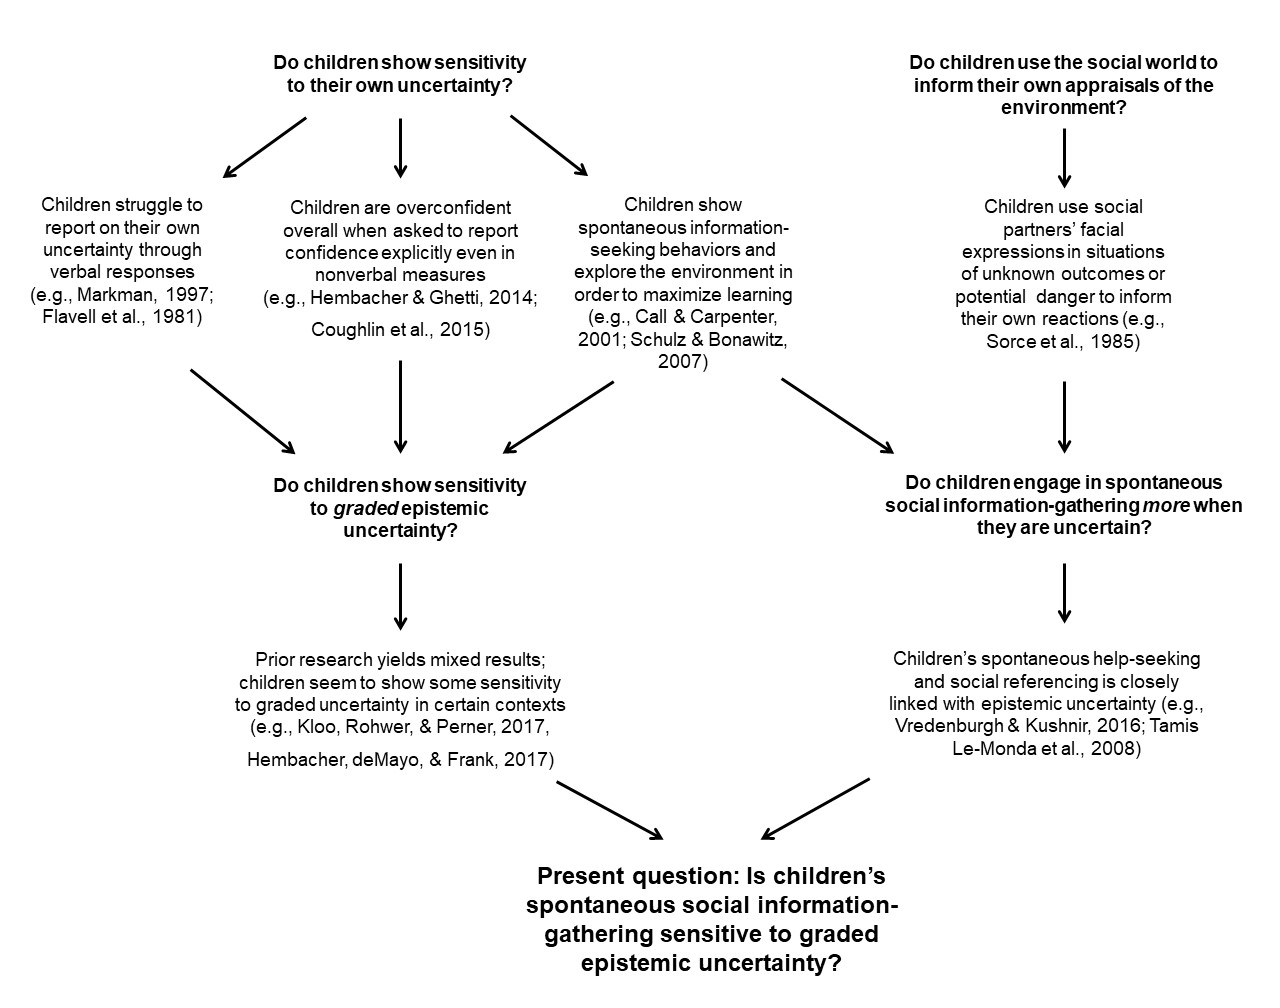
\includegraphics{../images/diagram_lit_review_1} 

}

\caption{Schematic representation of theoretical background and prior research informing the current study.}\label{fig:schematic}
\end{figure}

\#\#Uncertainty Monitoring and Active Learning in Early Childhood

Prior work on children's uncertainty monitoring has yielded mixed evidence as to whether young children can successfully recognize when they lack information and subsequently act on this knowledge of their own ignorance to make a decision (Sodian, Thoermer, Kristen, \& Perst, 2012). Early studies investigating metacognitive development indicated that children's competence in assessing and acting on their own epistemic ignorance is limited. Markman (1977) explained a card game to first and third grade children with ambiguous language such that understanding the object of the game was impossible without seeking clarification. An experimenter then prompted the child to seek this clarification with scripted statements such as \enquote{What do you think?}, \enquote{Do you have any questions?} and \enquote{Did I tell you everything you need to know to play the game?} In this study, Markman found that the younger children required more prompts before seeking out additional information, which she argues is an indication that young elementary school children do not engage in \enquote{constructive processing}. That is, they process the instructions being given by the experimenter superficially without simulating the process of trying to execute them, and are consequently unaware of gaps in their own knowledge.

Similarly, Flavell, Speer, Green, August, \& Whitehurst (1981) asked kindergarten and second-grade children to reconstruct block structures built by a confederate based on a tape of instructions from the confederate, which were not sufficiently clear to successfully recreate the structure. The researchers found that older children were more likely to indicate the need for additional clarifying information by replaying the tape, asking questions explicitly, or generally looking puzzled. Conversely, kindergarteners typically did not display these behaviors. This result demonstrated that older children were more adept at seeking information explicitly, but it also showed that younger children were less likely to spontaneously seek information from the environment (for example, by replaying the tape).

Rather than measure children's spontaneous information-seeking behaviors, some more recent research has gauged children's uncertainty monitoring capacities by asking them to report on their decision confidence in various contexts. When asked to report confidence in their answers on a memory task, 3-year-olds were equally confident about correct and incorrect responses, while 4- and 5-year-olds showed a more adult-like pattern of lower confidence for incorrect responses (Hembacher \& Ghetti, 2014). In a perceptual identification task, 3- to 5-year-olds reported being less confident when they provided incorrect responses, although overall they were still overconfident (Coughlin, Hembacher, Lyons, \& Ghetti, 2015). In order to avoid requiring a verbal response from children, which may obscure children's capacities to reflect on their own ignorance, these studies used a pictorial confidence scale when prompting children to report on their uncertainty. However, the possibility exists that even these studies underestimate children's ability to monitor their own uncertainty because they require children to explicitly report their confidence (even if not in an open-ended verbal response), and that children can act on their own uncertainty before they can communicate it through explicit responses or reflect on it consciously. Thus, although these studies did not hinge on an verbal report of uncertainty from children (which may be the most difficult response for a child to provide), they nonetheless required children to explicitly report on their confidence - a measure of uncertainty which may be still more difficult than more implicit, spontaneous and action-based measures.

\hypertarget{childrens-spontaneous-information-seeking-behaviors}{%
\subsection{Children's Spontaneous Information-Seeking Behaviors}\label{childrens-spontaneous-information-seeking-behaviors}}

In contrast to the explicit confidence measurements used in the studies discussed above, some research has shown that children engage in spontaneous information-gathering behaviors -- that is, behaviors that are not prompted explicitly by an experimenter -- more often when they are faced with uncertainty. These studies demonstrate that children engage in \emph{active learning}, in which the learner decides what information they want to be exposed to, rather than having the decision made for them by a teacher (Gureckis \& Markant, 2012). While early research on children's metacognitive development also measured unprompted information-seeking behaviors and found that younger children do not engage in spontaneous information-seeking, these early studies often required an explicit verbal response from children, as in Markman (1977). Furthermore, studies such as Flavell, et al. (1981) showed children's deficit in realizing when instructions are insufficient, which may be more difficult for children than realizing they lack other types of knowledge, such as memory of an event. Specifically, it may be particulary difficult for children to realize they lack understanding or knowledge of instructions, since doing so requires that children recognize that they may encounter an obstacle in the future which may not be immediately apparent to them at the moment the instructions are given.

Recent research which at least partially alleviated these task demands has found evidence of children's engagement in spontaneous information-seeking. In one study, when 2-year-old children were asked to find a sticker hidden inside of one of several tubes, they peeked inside the tubes more when they had not seen the experimenter place the sticker, indicating that they spontaneously sought out more information when deprived of sufficient information to make a decision (Call \& Carpenter, 2001). In another study, young children were shown a group of toys that either differed in their color or in how they felt to the touch (Robinson, Haigh, \& Pendle, 2008). All of the toys were put into a bag by the experimenter, who mixed them up and then picked out a toy. In the condition where the experimenter put the toy on the table and asked the child, \enquote{Which one is it?}, children more often reached out and touched the toy more when its distinctive quality was texture than when it was color. In contrast, when the experimenter handed the object to the child, thus giving the child visual and tactile access to the toy simultaneously, children still correctly were able to identify whether the toy was soft or hard, but unable to accurately report that they had arrived at this conclusion by touching the toy. Thus, in this particular context, children interacted with the environment using sensory modalities that most effectively filled in gaps in uncertainty, even if they were unable to explicitly report doing so.

Schulz and Bonawitz (2007) also found that when young children were presented with a causally-confounded toy (i.e., a toy that exhibited a behavior whose causal structure could not be deduced) and could choose between playing with that toy or a novel toy, they chose to further explore the causally-confounded toy. However, when the choice was between continuing to play with a causally-unconfounded toy and playing with a new toy, children preferred the novelty of exploring the new toy, demonstrating that children play spontaneously in order to maximize learning based on uncertainty about the world.

\#\#Children's Social Referencing and Social-Information Gathering

Taken together, these studies provide compelling evidence that children choose to seek information specifically to resolve uncertainty, and that they sample sources of evidence that are most likely to provide disambiguating information. In this study, I examine the selectivity of children's spontaneous sampling of social information. In order to do this, children must consider other people to be helpful sources of information.

Evidence in a number of experimental contexts suggests that infants and young children reference trusted adults for disambiguating information in situations of uncertain outcomes and potential danger. Sorce, Emde, Campos, and Klinnert (1985) showed that infants look to their mothers to determine whether it is safe to proceed crawling over a \enquote{visual-cliff}, a glass table that is actually safe to walk on but which looks like a daunting drop-off to an infant. When infants' caregivers showed an encouraging expression, infants tended to crawl onto the glass surface, whereas they avoided doing so when their mother showed a frightened facial expression. Other studies have shown that children use caregivers' emotional appraisals of novel toys (Feinman, 1982; Hornik, Risenhoover, \& Gunnar, 1987; Klinnert, 1981) and recently-met strangers(Feinman \& Lewis, 1983) to inform how they interact with newly-encountered aspects of their environments.

The above studies provide strong evidence that children, starting in the early stages of infancy, use others' appraisals of the world around them to resolve uncertainty about the safety or physical affordances of the environment. Specifically, they use information gleaned by looking at their social partners' faces to guide their own actions. Children, beginning in infancy, also reference speakers' gaze in order to determine the referent of a utterance, suggesting that looking to others' faces is a critical form of minimal infomation-seeking in early childhood (Baldwin, 1991). However, there is only limited prior research that sheds light on whether children's searches for social information are driven by gaps in the child's knowledge and their own awareness of these gaps.

There are several reasons to suspect that children may be less selective with their social information-seeking than they are with information-seeking in non-social contexts. Some forms of social information-seeking, such as looking at others' faces, may be less costly than other forms of manual exploration of the environment such as tactile play, in that they may require less time and cognitive resources. Additionally, social information may be sufficiently salient such that children sample it regardless of the uncertainty associated with a particular situation. This possibility is plausible given research which demonstrates that children focus more attention to faces and other socially informative aspects of complex scenes beginning as early as preverbal infancy (Frank, Vul, \& Johnson, 2009; Frank, Vul, \& Saxe, 2012). Nevertheless, prior research has shown that children show selectivity in some of their social information-gathering behaviors. Below, I review studies that demonstrate that children are selective when choosing their informants, and that they more heavily weight social information in situations of uncertainty.

\#\#Selective trust in testimony

A large body of evidence suggests that young children are selective social learners in terms of whom they choose as their informants. Younger children tend to use an informant's familiarity as a cue to the trustworthiness of the information being offered, but children gradually shift to depend more on an informant's demonstrated competence and expertise as they grow older (Corriveau \& Harris, 2009; Lucas, Lewis, Pala, Wong, \& Berridge, 2013). In one study, children were found to generally be proficient at tracking the accuracy of an informant's information when explicitly probed. Furthermore, children who showed this proficiency selectively learned novel object labels from an accurate informant, while those who failed to discriminate between an accurate and inaccurate informant likewise did not selectively use information from the accurate informant (Koenig, Clément, \& Harris, 2004). Children also show selective learning from an informant who appears uncertain versus one who is clearly knowledgeable, and are able to assess someone else's knowledge on a particular topic beyond perceptual cues such as facial expression (Sabbagh \& Baldwin, 2001). Taken together, these studies show that children, beginning in the preschool years, choose their information sources in order to maximize knowledge gain. However, it remains unclear whether children are similarly selective in their social information-gathering depending on their own level of epistemic ignorance.

\#\#Selective social learning on the basis of uncertainty

Despite young children's apparent lack of ability to explicitly report their own uncertainty, a few studies indicate that young children may seek and use information selectively from other people on the basis of epistemic uncertainty. Tamis-LeMonda et al. (2008) extended the finding of Sorce et al. (1985) in order to determine whether children consider the expressions of their caregivers more when the safety of the environment is more uncertain versus when it is completely certain. In this study, researchers tested whether 18-month-old infants would walk down slopes of varying risk levels when given either encouraging or discouraging signals from their mothers. The researchers found that children tended to ignore their mothers' encouraging messages when faced with a slope that was clearly too steep to walk down safely, and similarly ignored mothers' discouraging messages when the slope was obviously safe. At borderline slopes, when it was unclear to infants whether the slope was safe to walk down or not, children tended to comply much more consistently with the encouragement or discouragement provided by their mother, showing that even infants selectively give more weight to social information when perceptual input is not enough to make a decision.

While the study by Tamis-LeMonda et al.~examined children's selective integration of social information, it did not include children's sampling (e.g., through gaze shifts) of social information as a dependent measure. Some recent research has begun to address the question of whether children actively seek out information from their social partners when uncertainty is high. Vredenburgh and Kushnir (2016) investigated children's propensity to ask questions when faced with toy-assembly tasks of differential levels of difficulty. They found that preschoolers were significantly more likely to ask an experimenter for help on tasks that were more difficult for them, indicating that children adjust their social information-gathering behavior to optimize their learning. Another study examined whether infants selectively reference their social partners' gaze when their social partner has uttered an ambiguous object label (Vaish, Demir, \& Baldwin, 2011). In this study, infants heard an experimenter produce a novel label when there were either two or one novel objects present. Infants looked up more at the experimenter when there were two objects present and the referent of the experimenter's label was thus ambiguous.

A later study by Hembacher, deMayo, and Frank (2017) sought to replicate and extend the finding of Vaish et al.~with preschool-aged children. In this study, children aged 2 - 5 years were presented with either one or two objects, heard a label produced by the experimenter, and asked to put the labeled item in a bucket. The number of objects (1 vs.~2) and their familiarity to the child were varied to manipulate referential ambiguity. Across two experiments, they found that children looked up at the experimenter more as they were making their choice when referential ambiguity was present. Specifically, children did the most looking at the experimenter when both objects were novel, did the least looking when both objects were familiar, and did an intermediate amount when one of the objects was familiar and one was novel. Additionally, when helpful gaze from the experimenter was included as a between-subjects manipulation, children looked up at the experimenter more when one object was familiar and one was novel, but only when helpful gaze was absent, suggesting that children's social referencing might be sensitive to graded levels of epistemic uncertainty. Thus, children are not only sensitive to states of complete ignorance and complete knowledge, but may also be sensitive to intermediate levels of evidence for a hypothesis.

\#\#Sensitivity to Graded Uncertainty

Although these results provide initial evidence that children seek social information on the basis of graded uncertainty, this study did not manipulate ambiguity in a continuous fashion, but rather presented children with only one intermediate level of uncertainty between complete certainty and complete ambiguity. In many learning contexts (i.e., category learning) many more degrees of ambiguity exist than complete certainty and complete ambiguity.

It is unclear whether young children are sensitive to intermediate levels of epistemic uncertainty, but some research suggests that their capacity to monitor graded uncertainty may be limited. Morgan, Laland and Harris (2015) asked children between the ages of 3 and 7 to determine which of two illustrated quantities was bigger; on some trials, the quantities were more similar to each other (i.e., the task was more difficult) than in other trials. After receiving feedback on their choice, children could either stick with their initial answer or change it. Children of all ages in the study seemed to be generally insensitive to their own uncertainty, evidenced by the fact that they tended to stick with their original answers regardless of the initial difficulty of the task. A possible explanation for this result is that children may have more trouble showing sensitivity to graded uncertainty when doing so requires that they break from a decision they already committed to, as compared to engaging in other forms of spontaneous information-seeking.

Another body of research has shown that children over the age of 3 can report on states of complete ignorance or complete knowledge when asked about an object that is being hidden (e.g., Wimmer, Hogrefe, \& Perner, 1988), meaning that when they are asked if they know which object has been hidden, they can accurately report on their own knowledge state if they have seen the hiding event (complete certainty) or have not seen any objects at all (complete ignorance). However, children of the same age struggle in \emph{partial exposure tasks}, in which they are shown two objects and told one of them will be hidden, but are not able to see which one ends up being hidden (Kloo \& Rohwer, 2012; Sodian \& Wimmer, 1987). In these situations, children tend to erroneously report that they know which object has been hidden, even though they had no visual access to the hiding event. Some studies, however, show that children as young as 2 or 3 years old engage in spontaneous information-seeking when faced with ambiguity in partial exposure tasks (Call \& Carpenter, 2001; Kloo, Rohwer, \& Perner, 2017).

In sum, while 3 to 6-year-old children struggle to demonstrate explicit or verbal reasoning about their own ignorance in partial exposure tasks, some studies show that children may engage in spontaneous information-gathering when they lack sufficient knowledge to make a decision. This prior research leaves open the question of whether children engage in selective social-information gathering that reflects a sensitivity to graded uncertainty.

\#\#Current Study

Building off the findings discussed above, the current study used a categorization paradigm to determine whether children's social information-gathering is driven by graded uncertainty. Children completed a category discrimination game in which they were introduced to two creatures, and told that each creature had a specific box that it was supposed to live in. They were then handed a number of images depicting creatures at various points on the perceptual continuum between the two prototype images to which they had initially been exposed, and were asked to put each creature in its correct box. The critical dependent measure was the duration of children's looks to the experimenter seated across the table from them, which I measured with an SMI RED-n eye-tracker. I predicted that children would look longer to the experimenter when attempting to categorize stimuli closer to the center of the perceptual continuum.

A categorization task was used here in part because category learning is a critical learning context in early childhood. Young children possess many mechanisms that facilitate category learning, including sensitivity to statistical regularities in the environment (Saffran, Aslin, \& Newport, 1996), sensitivity towards correlations of shared attributes among objects (Younger, 1985), and acute attention to perceptual features such as shape (Imai, Gentner, \& Uchida, 1994). Selectively seeking social information on the basis of graded uncertainty could be another such mechanism that aids in children's category learning. It is an open question whether children seek out disambiguating evidence when there is less evidence for an object's category membership.

Eye-tracking technology was used in this study to allow me to measure the duration of children's looks to the experimenter with greater precision than that afforded by hand-coding. Typically, research in social cognition that uses eye-tracking (particularly when it involves children) measures children's gaze patterns on a digital stimulus display such as a television screen which shows still or moving images (Gredebäck, Johnson, \& Hofsten, 2009). This is partially due to the fact that live-eye tracking with both children and adults is more difficult than using conventional eye-tracking displays. Nevertheless, some research suggests that social looking behaviors may differ slightly when a participant is engaged in a real social interaction as opposed to viewing a screen image of the same interaction (Risko, Laidlaw, Freeth, Foulsham, \& Kingstone, 2012). One study in particular suggests that an interaction with a live conversant draws more social gaze than a video display of a similar interaction, simply because a live conversation creates the potential for social interaction in ways that videos cannot (Laidlaw, Foulsham, Kuhn, \& Kingstone, 2011). A separate line of research also shows that children learn more effectively when interacting with a social partner whose actions are contingent on the child's actions, as compared to watching a video of a person acting as a teacher (Roseberry, Hirsh-Pasek, \& Golinkoff, 2014; Troseth, Saylor, \& Archer, 2006). As a result, it may be that children shift gaze to a socially contingent partner in a different way than they would to a prerecorded social partner who does not actually interact with the child.

Despite the methodological challenges associated with live eye tracking, its use with children and infants is not unprecedented. This technique has mostly been used to examine social gaze irregularities in children with Autism Spectrum Disorder (ASD), and has been used with children of preschool and primary school age (Falck-Ytter, Carlström, \& Johansson, 2015; Nadig, Lee, Singh, Bosshart, \& Ozonoff, 2010; Noris, Nadel, Barker, Hadjikhani, \& Billard, 2012). At least one study has also extended this type of eye-tracking to typically-developing infants. Gredeback, Fikke, and Melinder examined the development of infants' gaze-following behaviors between 2 and 8 months using a live eye-tracking paradigm (2010). In this study, infants began showing gaze-following behaviors between 2 to 4 months of age, and were more likely to follow the gaze of a stranger than the gaze of their mother.

In sum, since prior research indicated that such a live eye-tracking approach was possible, and since using an eye tracker decreases the potential for human error involved in hand-coding, I used an eye-tracking setup to measure gaze shifts to an in-person social partner.

\hypertarget{methods}{%
\section{Methods}\label{methods}}

\hypertarget{pilot-testing}{%
\subsection{Pilot Testing}\label{pilot-testing}}

I developed the experimental procedure descibed below over a 5-week pilot testing period. During this period, I recruited 40 child participants at the Children's Discovery Museum in San Jose, CA who participated in various preliminary versions of the task. The primary purpose of pilot testing was to arrive at a version of the test that (a) showed levels of accuracy on the task that indicated differential levels of uncertainty for children, and (b) kept children engaged and (c) was enjoyable to them. Several facets of the experimental design were adjusted throughout the pilot-testing process, including the color of the stimuli, the number of trials, the presenation of motivational rewards (stickers) throughout the task, and whether children had visual access to prototype images of stimuli they were being asked to categorized during test trials.

\hypertarget{participants}{%
\subsection{Participants}\label{participants}}

I recruited a sample of 37 children aged 3 to 5 years (mean age = 4.61) at the Bing Nursery School at Stanford University in Stanford, CA. Seven children were dropped from the analyses because of issues with their data (e.g., incomplete video data or insufficient eye-tracker calibration). One child's data was formatted incorrectly, though I was not able to identify the source of the issue, so I had to drop the participant, leaving me with a final sample size of 29 participants (1 fewer than I specified in my preregistration, which can be found at \texttt{https://aspredicted.org/see\_one.php?a\_id=8960}). I asked all participants if they wanted to play a short game during their regularly scheduled free-play. Children were predominantly white and Asian and generally had highly-educated parents. All children were tested by the same experimenter (myself) and were randomly assigned to one of four counterbalance conditions.

\hypertarget{stimuli-design-and-procedure}{%
\subsection{Stimuli, Design and Procedure}\label{stimuli-design-and-procedure}}

\begin{figure}

{\centering 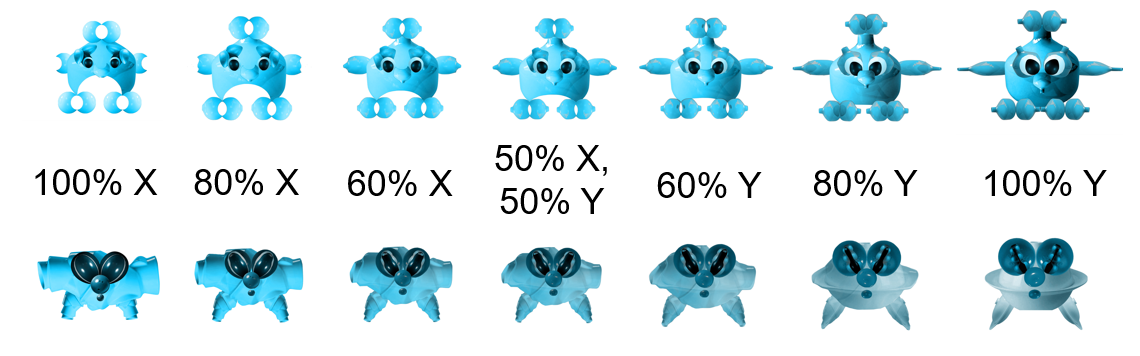
\includegraphics[width=3.8in]{../images/stimuli_1} 

}

\caption{Stimulus sets provided to children. Images on the ends of the spectrums are prototypes which morph into each other on a perceptual continuum.}\label{fig:stimuli}
\end{figure}

\hypertarget{a-stimuli.}{%
\subsubsection{a) Stimuli.}\label{a-stimuli.}}

Stimuli were slightly altered versions of those created by Havy and Waxman (2016). Havy and Waxman created their stimulus sets by rendering two novel prototype images and using Norrkross MorphX to create a perceptual continuum of stimulus items that were different morph combinations of the two prototypes. Since pilot testing revealed that the current task was too easy for children when the prototypes varied in color, I transformed them to be monochromatic blue (Figure \ref{fig:stimuli}). The images were printed and laminated to make rectangular cards that children could insert into one of the two boxes.

\hypertarget{b-experimental-setup-and-eye-tracking-mechanism.}{%
\subsubsection{b) Experimental Setup and Eye-tracking Mechanism.}\label{b-experimental-setup-and-eye-tracking-mechanism.}}

\begin{figure}
\centering
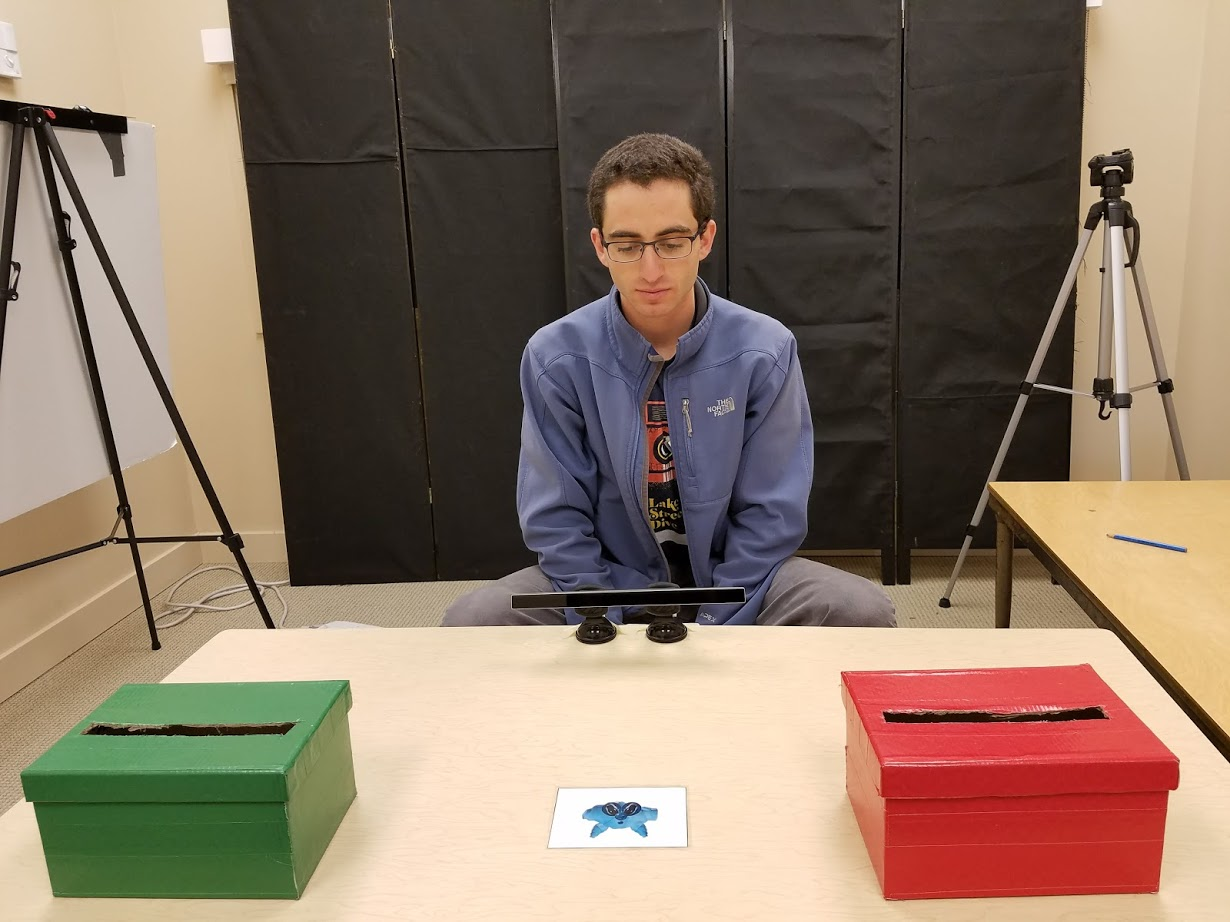
\includegraphics{../images/setup.jpg}
\caption{\label{fig:setup}Experimental setup from child's perspective. The eye-tracker across the table recorded gaze shifts to the experimenter throughout the task.}
\end{figure}

Children were seated in a small chair in front of a table which contained two boxes, one red and one green, both placed within their reach (Figure \ref{fig:setup}). The boxes had openings in the lids to allow children to deposit the stimulus cards into them. When children entered the room, they sat across a 60-centimeter-wide table from a large poster-board which displayed the images for the eye-tracking calibration procedure. After the calibration phase had ended and the experimental trials began, the poster-board was replaced with the experimenter sitting in a chair across the table from the child.

I used an SMI REDn corneal reflection eye-tracker to measure children's gaze shifts to the experimenter throughout the task. The eye-tracking device was placed on two magnetic mounts in the middle of the table, approximately 58 centimeters in front of the child. The child's field of vision was captured by an external-viewing webcam situated directly behind and slightly above the child's head.

\begin{figure}
\centering
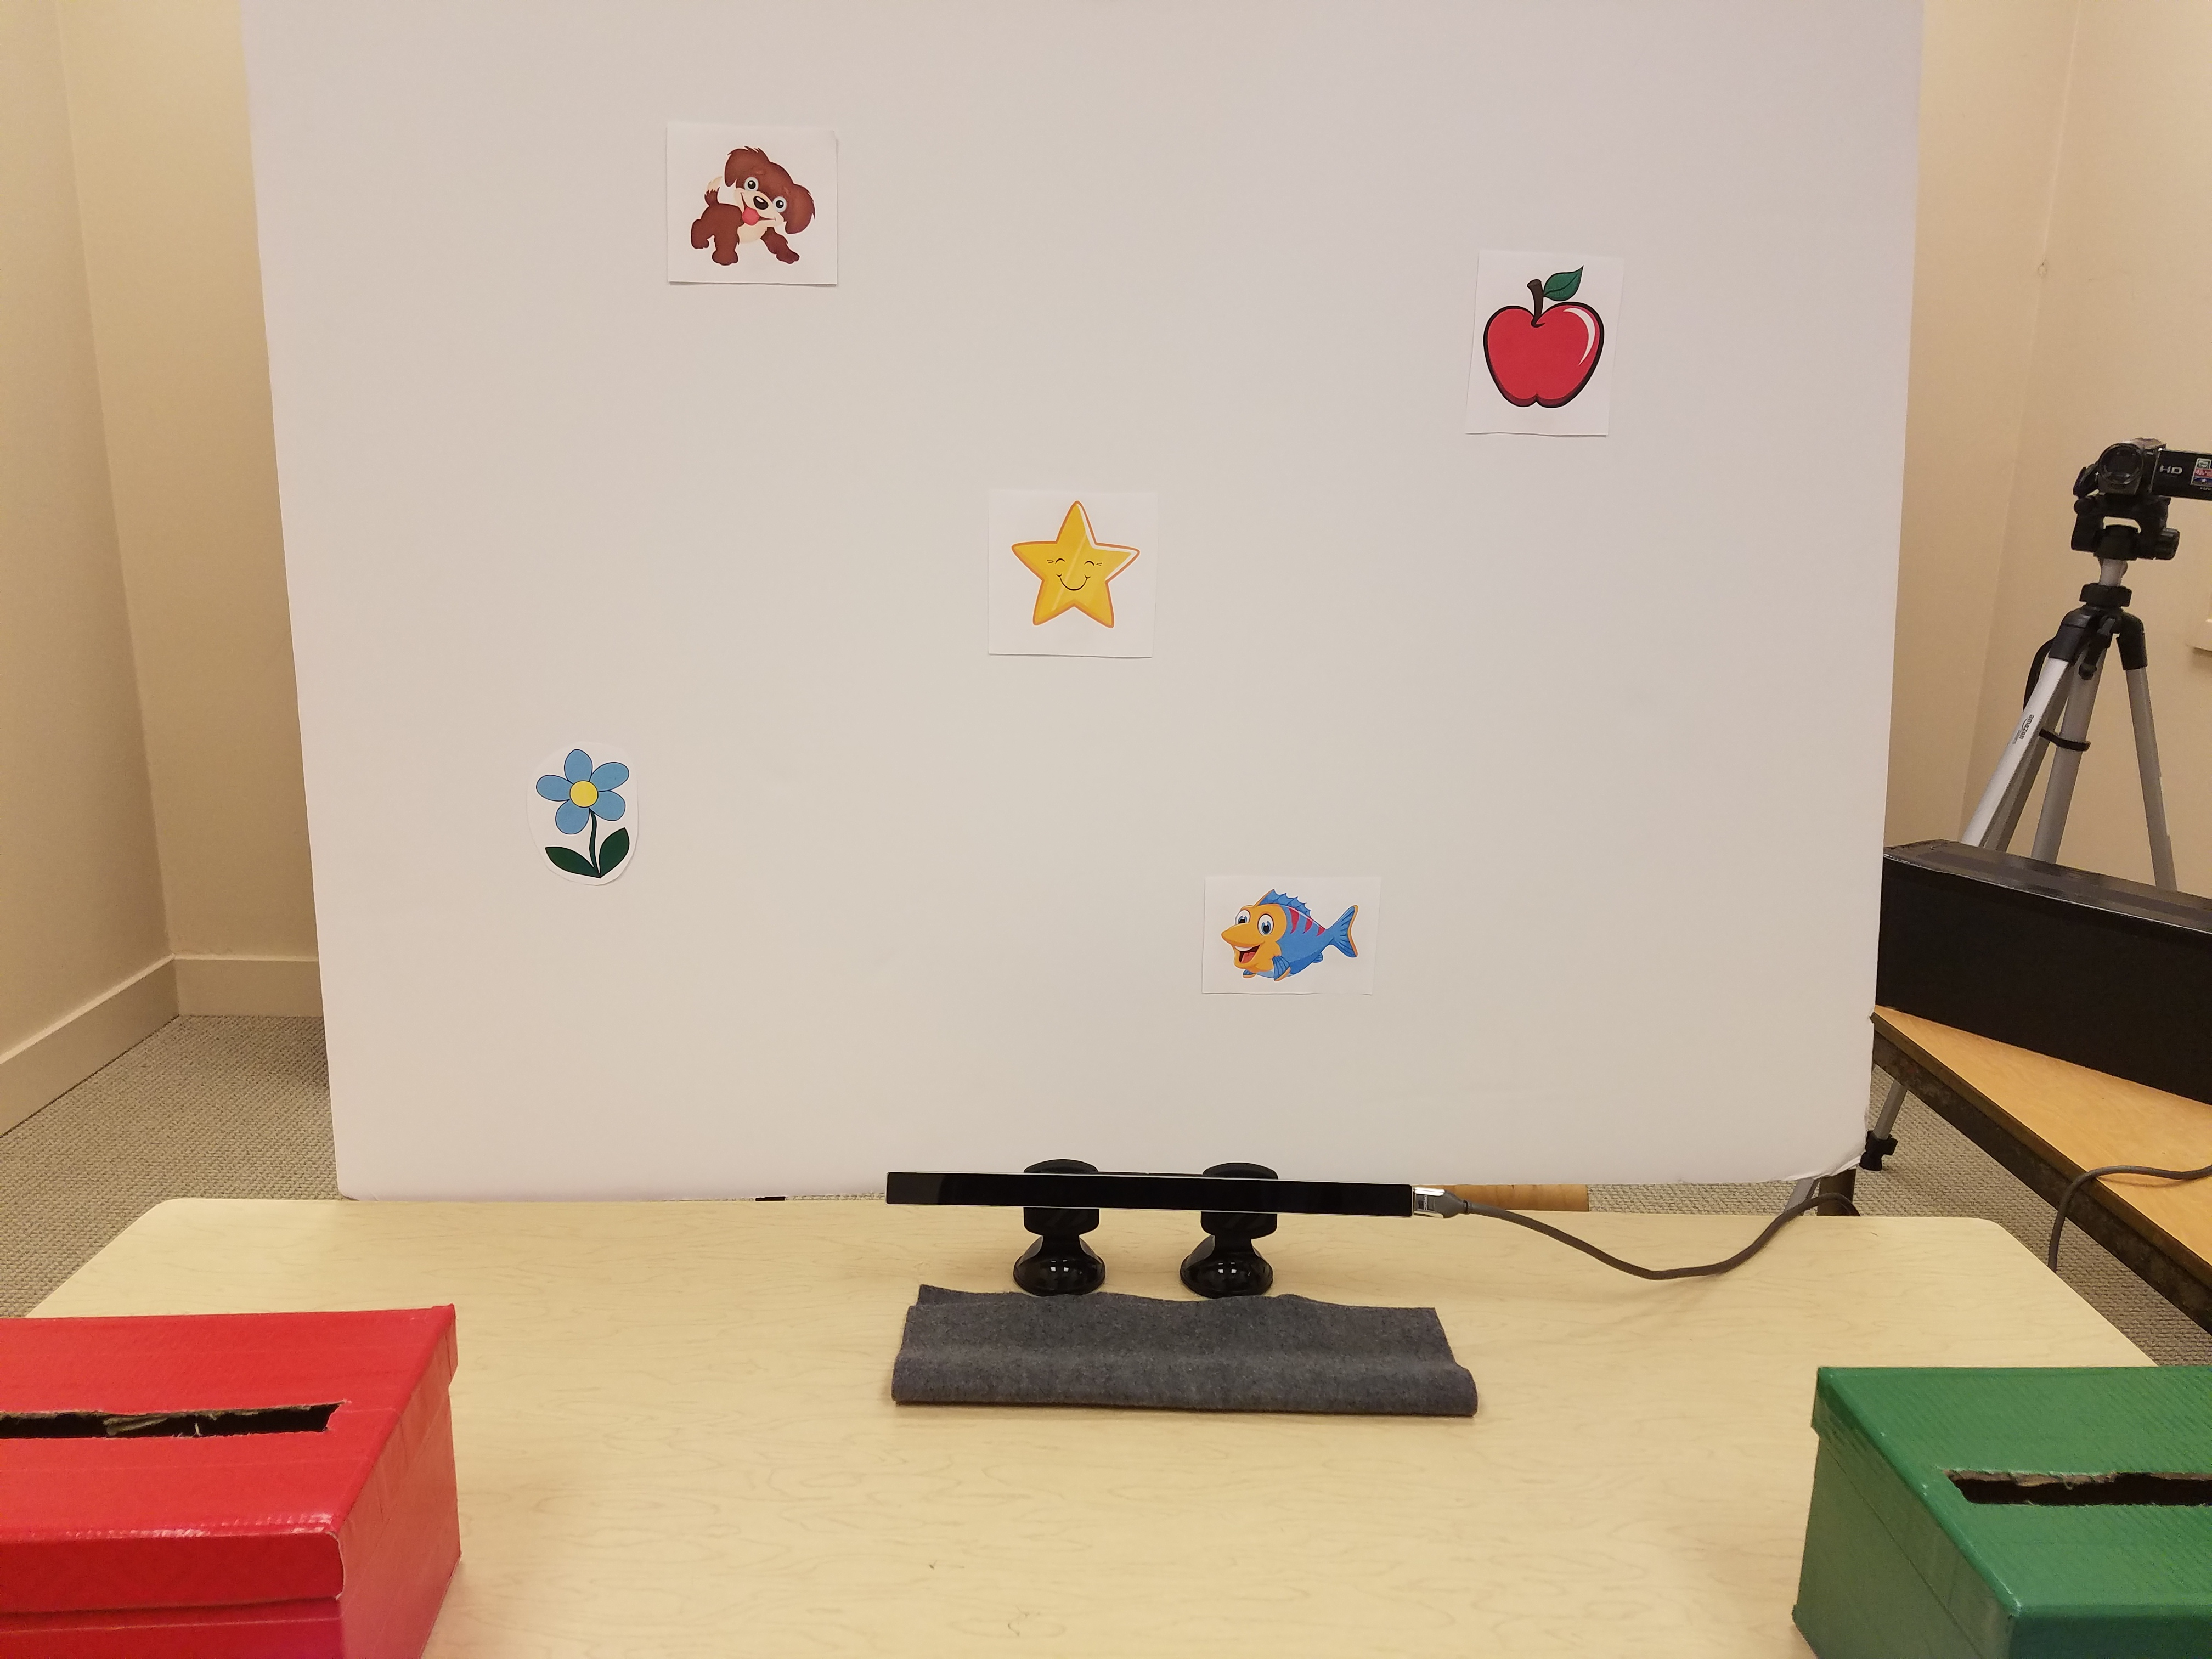
\includegraphics{../images/calibration.jpg}
\caption{\label{fig:calibration}Calibration display. During the calibration phase, children were directed to look at each image as the experimenter approved each calibration point one by one.}
\end{figure}

\hypertarget{c-calibration.}{%
\subsubsection{c) Calibration.}\label{c-calibration.}}

Children were directed to look at each of the 5 calibration images on the poster-board situated across the table from them while I approved each point one-by-one (Figure \ref{fig:calibration}). The calibration display consisted of a large white poster board with five cartoon images: a smiling star, a puppy, a blue fish, a flower, and a red apple. After I had approved each calibration point, the child was asked to follow my finger as it moved across the calibration display while I checked to see whether the eye-tracker was accurately representing the gaze location of the child. If I deemed this informal test of calibration accuracy to be sufficient, the experiment continued; if not, calibration was repeated.

\hypertarget{d-procedure.}{%
\subsubsection{d) Procedure.}\label{d-procedure.}}

Upon entering, I introduced children to a \enquote{sticker chart} that would be used throughout the task to keep them motivated and prevent them from getting fatigued during the experiment, which lasted about 12 minutes. Each child was asked if they preferred to write their name or whether they wanted my help in doing so; this introductory sequence was used as an opportunity to build rapport with each individual child. After the name was written on the chart, the calibration phase began.

Once the calibration phase was finished, I removed the poster board and sat across from the child. I then explained to the child that I had brought pictures of imaginary creatures with me, and that I needed the child's help putting them back in their boxes. The child then categorized six practice items: two items of a 90\% morph, two items of a 55\% morph, and two items of a 95\% morph. After the practice trials, the child completed 2 blocks of 7 test trials, each of which consisted of a 50\% morph (completely ambiguous) and two each of 60\%, 70\%, and 100\% morphs (identical to the prototypes). The morphs were presented in one of four pseudo-random orders that were counterbalanced across participants. After the first two test blocks, the child was introduced to a new pair of prototype creatures and asked to complete the same task with these new creatures. They then completed two new test blocks with the new set of creatures, consisting of the same ambiguity levels as the first two test blocks. In total, there were 6 practice and 28 test trials per child. In between each test or practice block, children got to choose a sticker for the chart they had made at the beginning of the experiment and were then reminded of the two prototype creatures at each end of the perceptual continuum. Pilot testing indicated that this procedure invoked differential levels of accuracy based on stimulus ambiguity and avoided performance degradation by continually re-introducing the prototypes and offering a motivational reward after each block of 7 trials.

\hypertarget{analysis}{%
\subsubsection{Analysis}\label{analysis}}

Each session was videotaped on a camera behind the experimenter's seat, allowing for view of the entire experimental setup. I hand-coded accuracy and trial onsets/offsets using DataVyu software (\texttt{http://datavyu.org}). I defined a trial as the span of time between when the stimulus item became available to the child (i.e., the experimenter let go of it) and when the item was deposited in a box. Accuracy was determined by whether a child placed the stimulus item in the box corresponding to the prototype it was closer to on the spectrum; therefore, stimuli that were an exact 50\% morph of both prototypes were not coded for accuracy. All stimuli, data, and analyses are available at \texttt{https://github.com/benjamindemayo/soc\_ref\_category}.

\hypertarget{results}{%
\section{Results}\label{results}}

\hypertarget{procedural-and-manipulation-checks}{%
\subsection{Procedural and Manipulation checks}\label{procedural-and-manipulation-checks}}

\begin{figure}
\centering
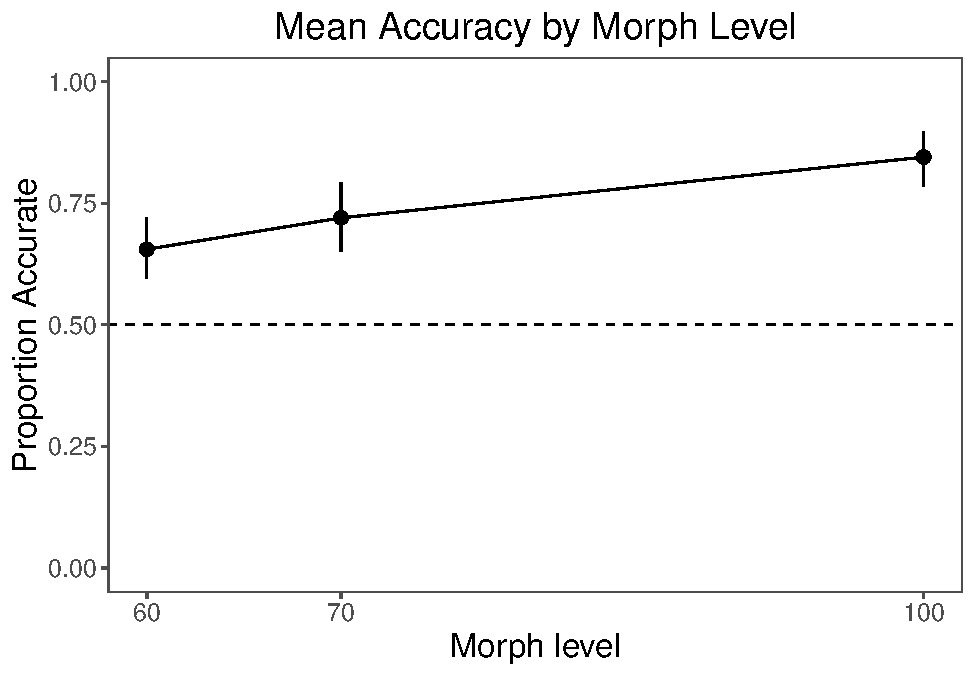
\includegraphics{soc_ref_category_paper_files/figure-latex/morphaccuracy-1.pdf}
\caption{\label{fig:morphaccuracy}Categorization accuracy for each morph level. Error bars are 95 percent confidence intervals.}
\end{figure}

\begin{table}[ht]
\centering
\caption{Results from logistic regression model predicting children's categorization accuracy.} 
\begin{tabular}{lrrrll}
  \hline
Predictor & Estimate & Std. Error & $z$ value & $p$ value &   \\ 
  \hline
Intercept & -1.00 & 0.47 & -2.14 & 0.03 & * \\ 
  Morph & 0.03 & 0.01 & 4.68 & $<$ .001 & *** \\ 
  Age & -0.95 & 0.87 & -1.10 & 0.27 &  \\ 
  Morph * Age & 0.02 & 0.01 & 1.43 & 0.15 &  \\ 
   \hline
\end{tabular}
\end{table}

\begin{figure}
\centering
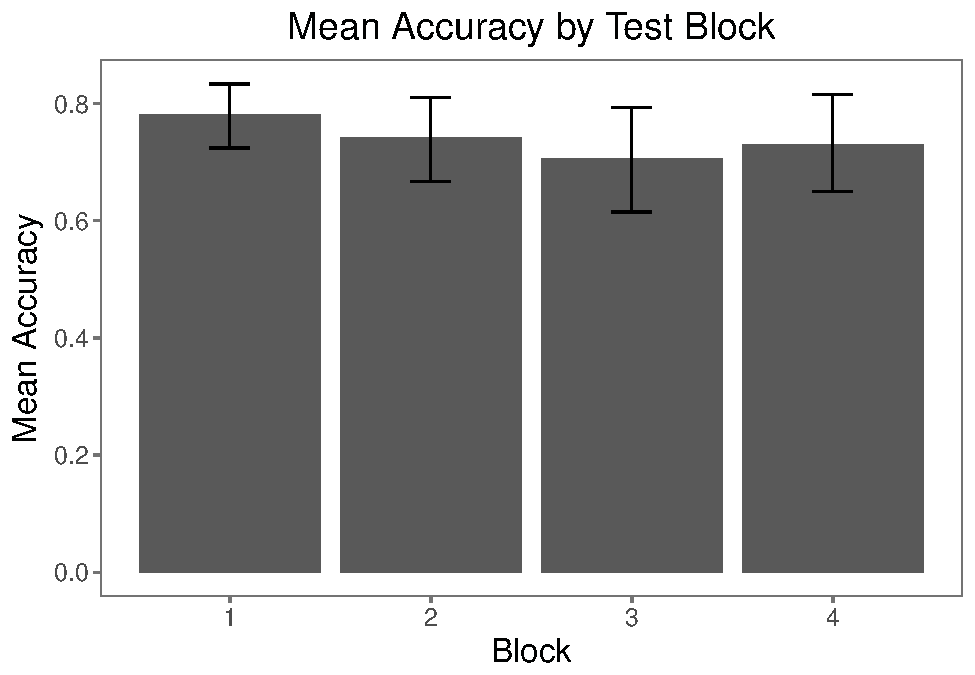
\includegraphics{soc_ref_category_paper_files/figure-latex/blockaccuracy-1.pdf}
\caption{\label{fig:blockaccuracy}Categorization accuracy for each of four experimental blocks, suggesting that children's accuracy did not degrade throughout the task. Error bars are 95 percent confidence intervals.}
\end{figure}

To validate the manipulation of category ambiguity in my procedure, I first examined whether children's accuracy on the categorization task (i.e., whether they put each item in the box of the prototype it was closer to) corresponded to the category ambiguity of each stimulus item (Figure \ref{fig:morphaccuracy}). Evidence from pilot testing indicated that children's accuracy on the task was highest for the least ambiguous stimuli, while children were least accurate when categorizing most ambiguous stimuli. To confirm this finding of the effect of morph level on accuracy, I first tried to fit the following logistic regression model to the data, which accounted for random effects (such as participant and trial number) denoted here and throughout the remainder of this report in parentheses: \texttt{accuracy\ \textasciitilde{}\ morph\ *\ centered\ age\ +\ (morph\ \textbar{}\ participant)\ +\ (1\ \textbar{}\ trial)}. Because this model did not converge, I pruned the model to remove the interaction effect between morph and participant, leaving me with the following model structure: \texttt{accuracy\ \textasciitilde{}\ morph\ *\ centered\ age\ +\ (1\ \textbar{}\ participant)\ +\ (1\ \textbar{}\ trial)}.

I found morph to be a significant predictor of children's accuracy such that stimulus items closer to the ends of the perceptual continuum were more likely to be categorized accurately, (\(\beta\) = 0.03, \emph{p} \textless{} .001). These results demonstrate that the task was more difficult for children when they were tasked with categorizing more ambiguous stimuli.

Additionally, as shown in Figure \ref{fig:blockaccuracy}, children's performance on the task remained consistent throughout the approximately 6 minute duration of test trials, indicating that children stayed engaged and motivated throughout the experiment. This is confirmed by the use of a logistic regression model of the structure \texttt{accuracy\ \textasciitilde{}\ block\ *\ centered\ age\ +\ (1\ \textbar{}\ participant)\ +\ (1\ \textbar{}\ trial)}, which found no significant effects of block on children's accuracy (\(p\) values for each level of \texttt{block} \textgreater{} 0.13).

\begin{figure}
\centering
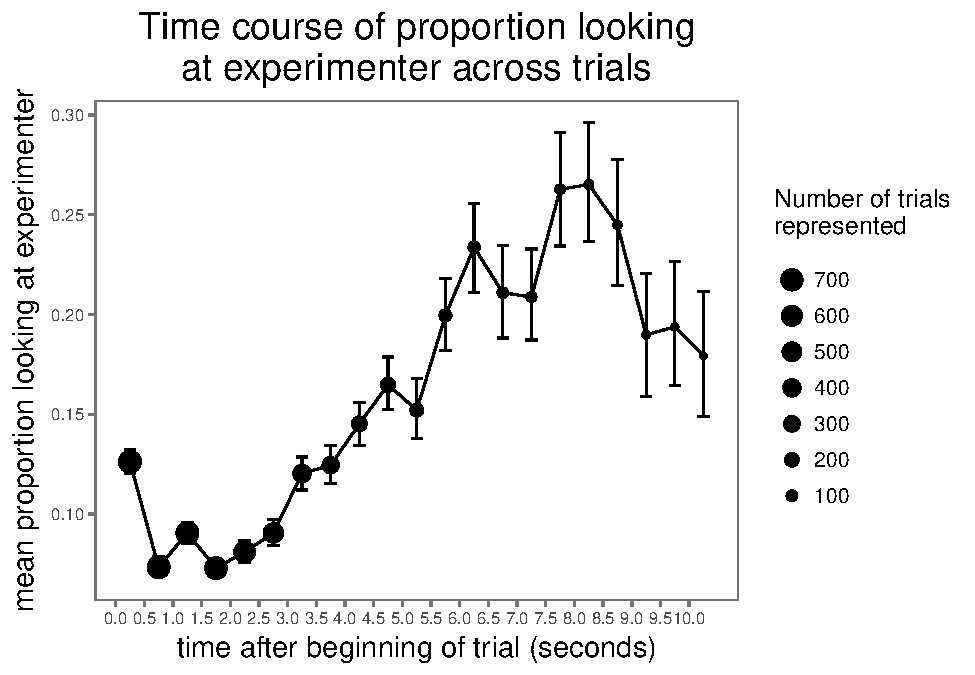
\includegraphics{soc_ref_category_paper_files/figure-latex/forwardtimecourse-1.pdf}
\caption{\label{fig:forwardtimecourse}Timecourse of proportion looking at experimenter, in half-second intervals. Size of points indicates amount of trials represented in each point. Dashed vertical line is median trial length. Error bars are 95 percent confidence intervals.}
\end{figure}

I examined the average timecourse of children's looking patterns during trials to ensure that data output from the eye-tracker was aligning appropriately with video data used to hand-code the onsets and offsets of each trial. Figure \ref{fig:forwardtimecourse} shows, for each half-second interval after the beginning of the trial, the average proportion of that interval that children spent looking at the experimenter, split by morph level (median trial length = 3.20 seconds). Since the eye-tracking data collection method in this paradigm was relatively imprecise due to the in-person interactive setup, any looks captured by the eye-tracker were considered to be a look in the general direction of the experimenter; thus, the \enquote{Area of Interest} in this design was defined as the entire spatial area for which the eye-tracker was calibrated.

\begin{figure}
\centering
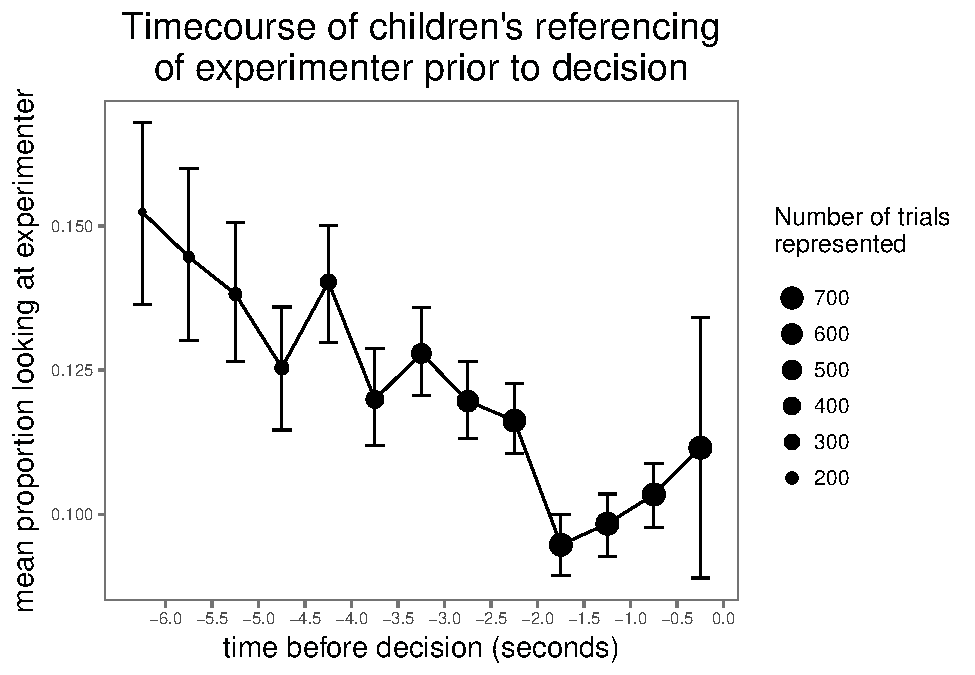
\includegraphics{soc_ref_category_paper_files/figure-latex/reversetimecourse-1.pdf}
\caption{\label{fig:reversetimecourse}Timecourse of children's looking at experimenter prior to decision, in half second intervals. Error bars are 95 percent confidence intervals.}
\end{figure}

In general, Figure \ref{fig:forwardtimecourse} shows that children tend to look slightly more at the experimenter at the very beginning of the trial, perhaps since this is when they are receiving the stimulus item from the experimenter. As trial length increases, so does the proportion of time in each half-second interval that children spend looking at the experimenter, which may be in part because longer trials frequently featured children asking questions and thus making eye-contact with the experimenter. Figure \ref{fig:reversetimecourse} shows the timecourse of children's looking in half-second intervals in relation to the end of the trial, which corresponds to the child's decision to place the stimulus item in one box or another. This plot shows a slight peak in children's looking behavior approximately 2 - 3 seconds before a decision. The general trajectories of children's eye-gaze in Figures \ref{fig:forwardtimecourse} and \ref{fig:reversetimecourse} are similar for all levels of morph, suggesting that differences in stimulus ambiguity did not lead to different patterns of looking during trials (see section on Proportion of Trial Looking by Morph for statistical tests of this result). Taken together, these plots provide some evidence that my data collection method captured a systematic pattern of looking with respect to the onsets and offsets of trials.

\#\#Response Latencies

\begin{figure}
\centering
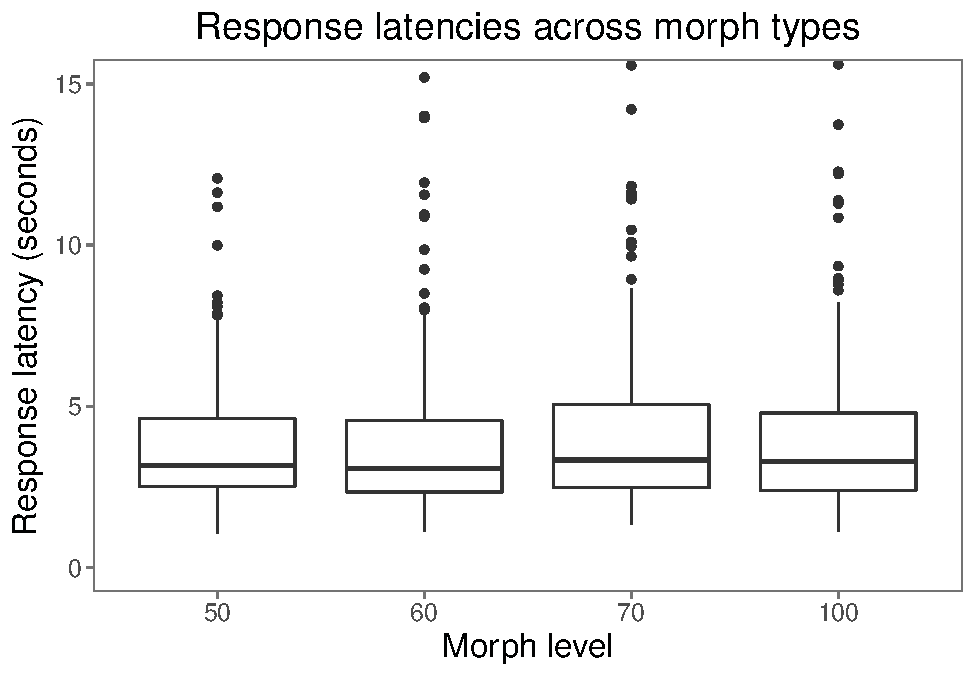
\includegraphics{soc_ref_category_paper_files/figure-latex/latencies-1.pdf}
\caption{\label{fig:latencies}Response latencies (trial length), which did not differ across stimulus items of different morph levels.}
\end{figure}

I examined the distribution of children's response latencies across each of the four morph conditions as a potential measure of children's uncertainty on the task. Response latency is defined here as the amount of time between the child gaining access to the stimulus item and their action of depositing it in one of the boxes. Figure \ref{fig:latencies} illustrates that there are no obvious differences between the distributions of response latencies for stimuli of different ambiguity levels. To confirm this finding, I used a linear mixed-effects model of the following structure to examine whether morph was related to response latency: \texttt{trial\_length\ \textasciitilde{}\ morph\ \ *\ centered\ age\ +\ (morph\ \textbar{}\ participant)\ +\ (1\ \textbar{}\ trial)}. I found no effect of morph on response latency (\(\beta\) = 0.00, \emph{p} = 0.59), indicating that children did not differ in their response latency depending on the ambiguity of the stimulus item they were asked to categorize.

\#\#Proportion of Trial Looking by Morph
Did children selectively seek out more social information when tasked with categorize more ambiguous stimulus items? I fit the data to a linear mixed-effects model to quantify the effect of category ambiguity on proportion of trial spent looking at the experimenter, along with any possible developmental trends. I first attempted to fit a linear mixed-effects model with the following preregistered structure: \texttt{proportion\ of\ trial\ spent\ looking\ \textasciitilde{}\ morph\ *\ centered\ age\ +\ (morph\ \textbar{}\ participant)\ +\ (1\ \textbar{}\ trial)}, with morph as a continuous variable. This model failed to converge, and so was pruned to remove the interaction effect between morph and participant. The resulting model had the following structure: \texttt{proportion\ of\ trial\ spent\ looking\ \textasciitilde{}\ morph\ *\ centered\ age\ +\ (1\ \textbar{}\ participant)\ +\ (1\ \textbar{}\ trial)}.

\begin{table}[ht]
\centering
\caption{Results from linear mixed-effects model predicting the proportion of trial duration children spent looking at the experimenter.} 
\begin{tabular}{lrrrll}
  \hline
Predictor & Estimate & Std. Error & $t$ value & $p$ value &   \\ 
  \hline
Intercept & 0.08 & 0.02 & 3.27 & 0 & ** \\ 
  Morph & 0.00 & 0.00 & 1.14 & 0.26 &  \\ 
  Age & -0.04 & 0.05 & -0.85 & 0.4 &  \\ 
  Morph * Age & -0.00 & 0.00 & -0.04 & 0.97 &  \\ 
   \hline
\end{tabular}
\end{table}

\begin{figure}
\centering
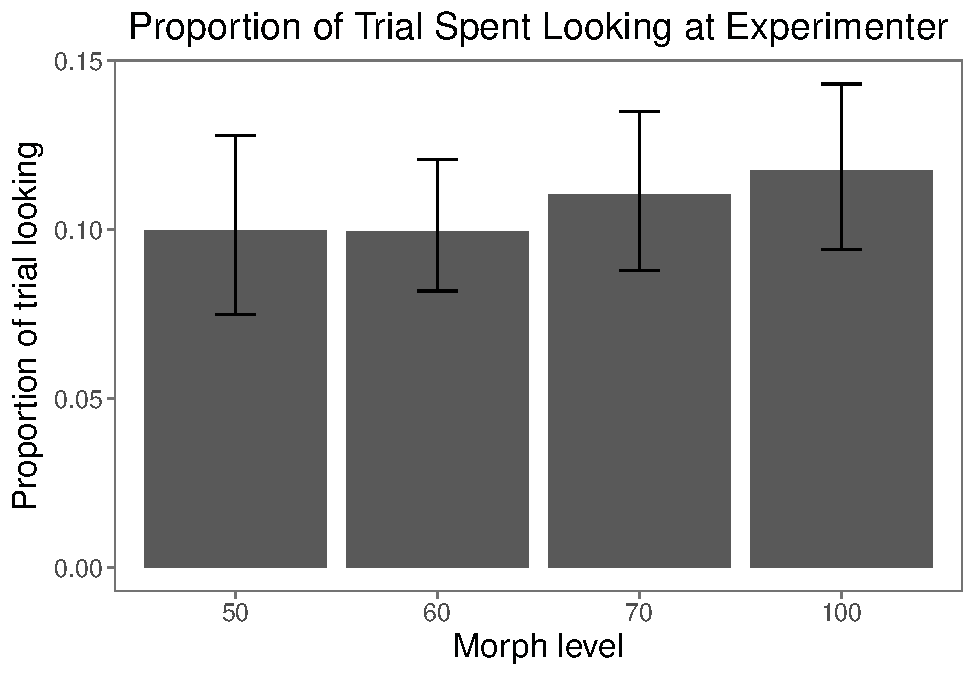
\includegraphics{soc_ref_category_paper_files/figure-latex/morphlooking-1.pdf}
\caption{\label{fig:morphlooking}Proportion of trial time spent looking at experimenter by morph level. Error bars are 95 percent confidence intervals.}
\end{figure}

\begin{figure}
\centering
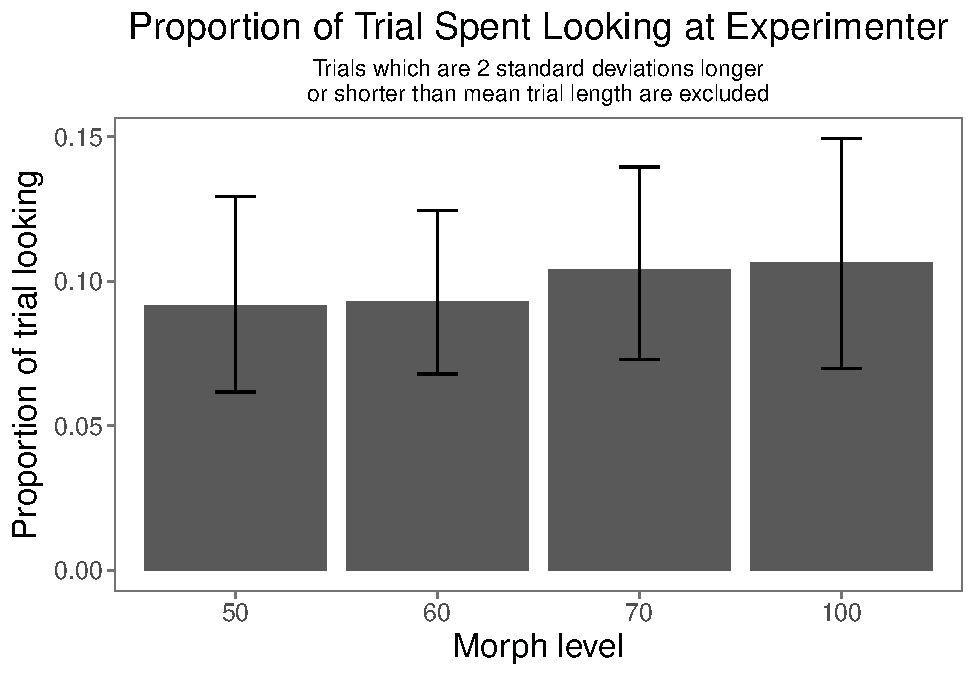
\includegraphics{soc_ref_category_paper_files/figure-latex/morphlookingtrimmed-1.pdf}
\caption{\label{fig:morphlookingtrimmed}Proportion of trial time spent looking at experimenter by morph level, excluding trials that are 2 standard deviations longer or shorter than the mean trial length. Error bars are 95 percent confidence intervals.}
\end{figure}

I found no effect of stimulus ambiguity (morph level) on the proportion of trial that children spent looking at the experimenter (\(\beta\) = 0.00, \emph{p} = 0.26), indicating that children did not selectively look longer at the exprimenter when faced with a more uncertain decision (Figure \ref{fig:morphlooking}).

As an exploratory analysis, I removed the age effect and interaction from the model, leaving me with the following model structure: \texttt{proportion\ of\ trial\ spent\ looking\ \textasciitilde{}\ morph\ +\ (1\ \textbar{}\ participant)\ +\ (1\ \textbar{}\ trial)}. I again found no effect of morph on proportion of trial duration spent looking (\(\beta\) = 0.00, \emph{p} = 0.26).

To verify that the results were not being skewed by a few extremely long trials, I also visualized the same analysis while excluding trials that were two standard deviations longer or shorter than the mean trial length. The looking pattern across various morph levels when excluding extremely long trials (Figure \ref{fig:morphlookingtrimmed}) is almost identical to the looking pattern observed without excluding any trials (Figure \ref{fig:morphlooking}), indicating that the presence of a few very long trials did not obscure a clearer pattern of referencing based on stimulus category ambiguity.

\hypertarget{narrowing-the-area-of-interest}{%
\subsubsection{Narrowing the Area of Interest}\label{narrowing-the-area-of-interest}}

\begin{figure}
\centering
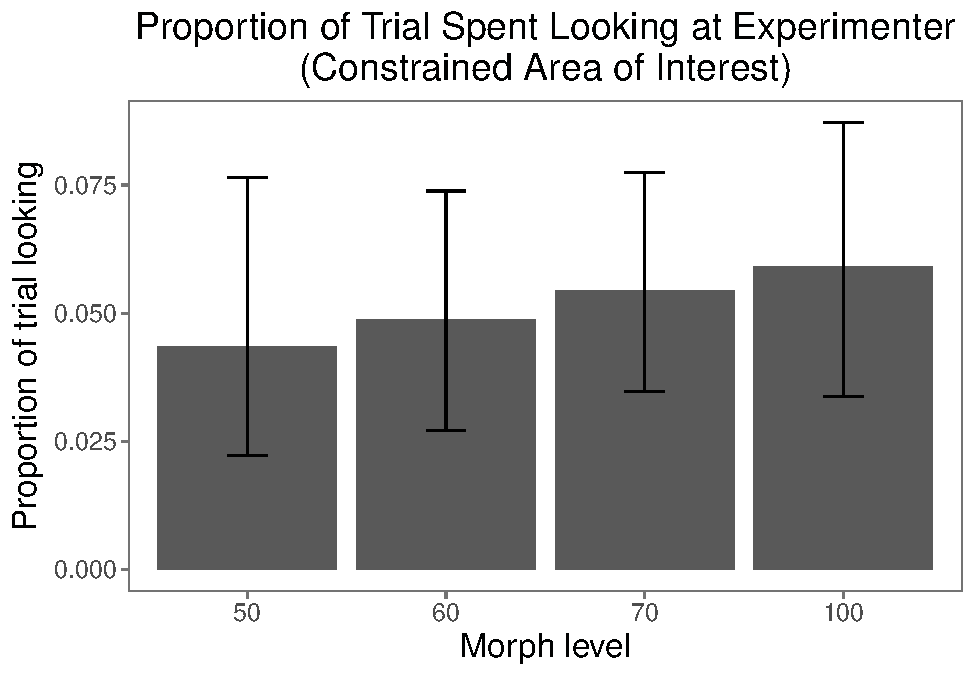
\includegraphics{soc_ref_category_paper_files/figure-latex/morphconstrained-1.pdf}
\caption{\label{fig:morphconstrained}Proportion of trial time spent looking at experimenter by morph level, constraining the area of interest to the middle half of the calibration area in the horizontal direction and the top two-thirds of the calibration area in the vertical direction. Error bars are 95 percent confidence intervals.}
\end{figure}

As an exploratory analysis, I narrowed the dimensions of the area-of-interest (AOI) to only include looks to the middle half of the calibration area (in the horizontal direction) and in the top two-thirds of the calibration area (in the vertical direction) in the analysis (Figure \ref{fig:morphconstrained}). I used a linear mixed-effects model with the same structure as the previous analysis and found no effect of morph level on proportion of trial duration children spent looking to the experimenter within the constrained area of interest (\(\beta\) = 0.00, \emph{p} = 0.18).

\begin{figure}
\centering
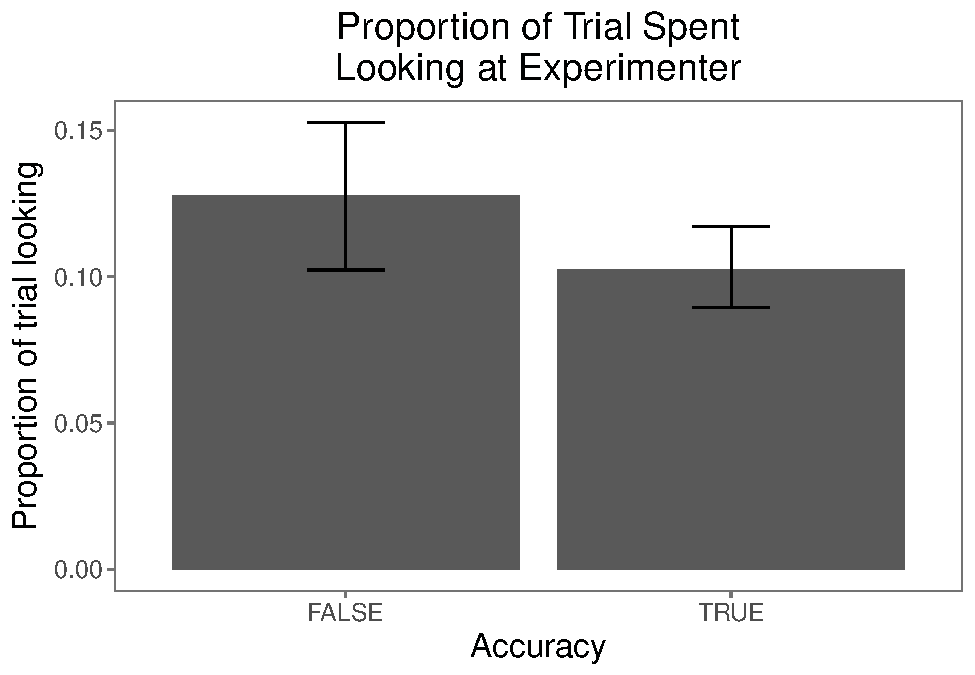
\includegraphics{soc_ref_category_paper_files/figure-latex/accuracylooking-1.pdf}
\caption{\label{fig:accuracylooking}Proportion of time during trials spent looking at experimenter by children's category accuracy. Error bars are 95 percent confidence intervals.}
\end{figure}

\hypertarget{proportion-of-trial-looking-by-task-accuracy}{%
\subsection{Proportion of Trial Looking by Task Accuracy}\label{proportion-of-trial-looking-by-task-accuracy}}

I also examined whether children's accuracy on the task was related to the proportion of time during trials children spent looking at the experimenter (Figure \ref{fig:accuracylooking}). To answer this question, I used a linear mixed-effects model with the following structure: \texttt{proportion\ of\ trial\ spent\ looking\ \textasciitilde{}\ accuracy\ *\ centered\ age\ +\ (accuracy\ \textbar{}\ participant)\ +\ (1\ \textbar{}\ trial)}. I found no effect of accuracy on proportion of time during trials spent looking at the experimenter (\(\beta\) = -0.01, \emph{p} = 0.32), indicating that children overall did not look at the experimenter more on trials when they were inaccurate versus accurate.

\begin{table}[ht]
\centering
\caption{Results from linear mixed-effects model predicting the proportion of trial duration children spent looking at the experimenter from trial accuracy.} 
\begin{tabular}{lrrrll}
  \hline
Predictor & Estimate & Std. Error & $t$ value & $p$ value &   \\ 
  \hline
Intercept & 0.11 & 0.02 & 6.60 & $<$ .001 & *** \\ 
  Accuracy (True) & -0.01 & 0.01 & -1.01 & 0.32 &  \\ 
  Age & -0.09 & 0.03 & -2.58 & 0.02 & * \\ 
  Morph * Age & 0.05 & 0.02 & 1.98 & 0.06 & . \\ 
   \hline
\end{tabular}
\end{table}

\begin{figure}
\centering
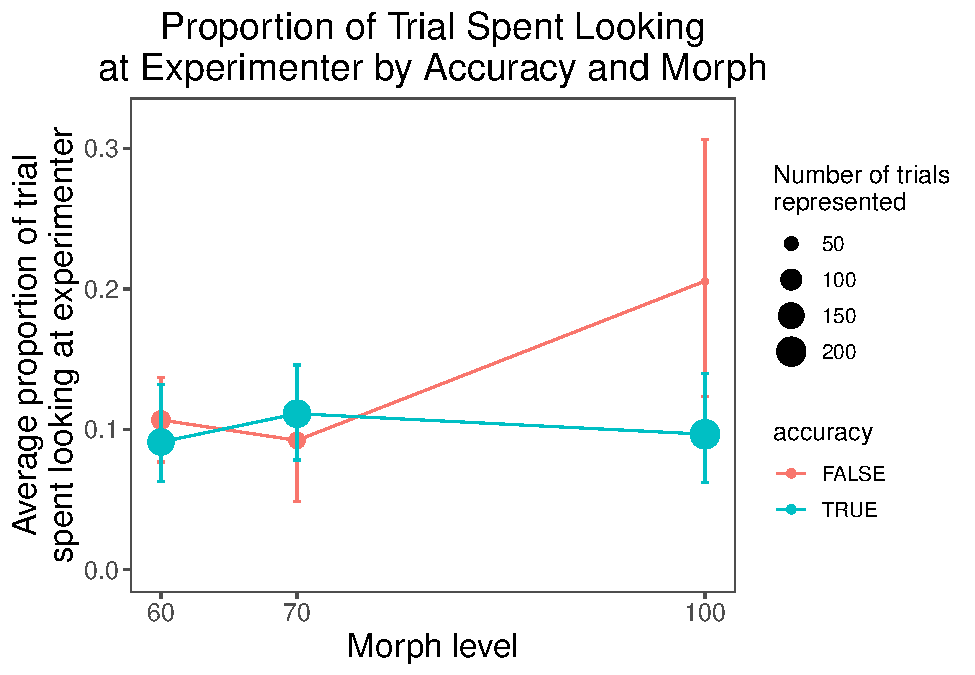
\includegraphics{soc_ref_category_paper_files/figure-latex/accuracylookingmorph-1.pdf}
\caption{\label{fig:accuracylookingmorph}Proportion of trial duration spent looking at the experimenter, by morph level and accuracy. When categorizing items of morph level 100 (exact prototypes), children who were inaccurate tended to look at the experimenter more.}
\end{figure}

Figure \ref{fig:accuracylookingmorph} shows an exploratory analysis that illustrates an interesting trend: on trials of morph level 100, children who categorized the item incorrectly seemed to look more at the experimenter than those who categorized the item correctly. To confirm the presence of this pattern, I used the same linear mixed-effects model as described above to determine whether accuracy is related to the proportion of trial duration that children spent looking at the experimenter, but I limited the analyses to trials of morph level 100. When the model was restricted to these morph-level-100 trials, I found that children looked at the experimenter for a significantly higher proportion of the trial when categorizing the items inaccurately versus accurately (\(\beta\) = -0.07, \emph{p} = 0.02). However, this result should be interpreted with caution, since there were relatively very few trials in which participants inaccurately categorized stimuli of morph level 100 (n = 36).

\hypertarget{discussion}{%
\section{Discussion}\label{discussion}}

In this study, I set out to understand whether children are sensitive to graded levels of uncertainty, and whether they would adjust their social-information seeking on the basis of this uncertainty. Previous research suggested that, while young children typically fail uncertainty monitoring tests that require explicit or verbal responses (Flavell et al., 1981; Markman, 1977), they explore environments in order to maximize their learning about the world (Schulz \& Bonawitz, 2007) and ask questions in order to extract useful information from knowledgeable social partners (Chouinard, Harris, \& Maratsos, 2007). These seemingly conflicting findings indicate that children's uncertainty monitoring capacities can be observed through spontaneous information-seeking behaviors before children can explicitly report on these capacities.

Indeed, several studies have shown that, beginning in infancy, children seek out information in ways that seem to be driven by uncertainty (Goupil, Romand-Monnier, \& Kouider, 2016; Vaish et al., 2011). Of particular interest to the current work, several studies have shown children's engagement in selective information-gathering when other people are the source of disambiguating information. When children seek information from the social world, the resulting interactions seem to reflect that the child is sensitive to their own uncertainty; moreover, prior research suggests that they leverage this sensitivity in order to strategically reference others when they need information, and do so less when they do not need information (Kushnir, Vredenburgh, \& Schneider, 2013; Vredenburgh \& Kushnir, 2016).

While prior work has shown that children spontaneously seek out social information on the basis of epistemic uncertainty, I aimed here to understand more about the relationship between children's social-information gathering and their sensitivity to graded levels of uncertainty. Empirical evidence has suggested that children may possess some sensitivity to graded evidence and intermediate levels of uncerainty in the environment, in such contexts as \enquote{partial exposure} tasks (Call \& Carpenter, 2001; Kloo et al., 2017) and word learning situations (Hembacher et al., 2017). Overall, however, very little is known about children's sensitivity to graded levels of uncertainty. It could be that children only show differential levels of spontaneous information-seeking from the social world when faced with situations of complete certainty versus complete ignorance.

Several aspects of this study design differ from previous research which investigated children's social information-gathering and uncertainty monitoring. Although this type of live-eye tracking paradigm has been used in numerous studies, particularly those investigating social gaze patterns in children with autism, it is still exceedingly rare among empirical research in developmental psychology. My principal motivation for using this eye-tracking setup here was to obtain information about the duration of children's gaze shifts to a social partner in a continuous interaction, which is difficult to quantify solely through a hand-coding mechanism. Moreover, to my knowledge, children's uncertainty as it relates to graded category ambiguity has not been previously investigated. In the current study, asking children to categorize ambiguous stimuli allowed me to experimentally induce conditions of graded uncertainty.

Given existing evidence of children's sensitivity to their own uncertainty, and their tendency to adjust their social interactions to selectively seek out information when faced with uncertainty, I hypothesized here that children would show a looking pattern that would indicate sensitivity to graded uncertainty, and would selectively seek more social information on trials in which they were tasked with categorizing more ambiguous stimuli. Contrary to my hypothesis, I found that children did not differentiate between trials of different morph levels in their amount of looking to the experimenter. A linear mixed-effects model demonstrated that stimlus ambiguity had no effect on the proportion of each trial that children spent looking at the experimenter. Thus, the data do not explicitly show that children possess sensitivity to graded levels of uncertainty, nor do they show that children strategically adjust the amount of social information they seek out on the basis of subjective uncertainty. If either of these constructs were visible in the data, then I would have observed a larger proportion of trial time spent looking at the experimenter when the stimulus items were more ambiguous. I did find a small difference in looking behaviors when children were categorizing the most unambiguous stimuli, such that children looked longer when they categorized these items incorrectly than they did when they categorized them correctly. I have no strong hypothesis as to why this trend appears in the data, although it may be related to the fact that children who categorized these items incorrectly were overall more uncertain during the task, and therefore engaged with the experimenter more often to ask for help. Regardless of the explanation for this finding, I encourage interpreting it with caution, since such a small number of children miscategorized the morph-100 level stimuli.

Interestingly, I also found no difference in looking behaviors even between trials which were completely ambiguous (morph level 50) and trials which were identical to the prototypes shown to children at the beginning of each experimental block (morph level 100). This result is particularly striking given that children were significantly less accurate in categorizing more ambiguous items, indicating that task difficulty was not uniform across trials. This finding contrasts that of Hembacher, deMayo, and Frank (2017), who found that, in a word-learning task, children's social information gathering was closely linked to referential ambiguity. What might be the origin of the discrepancy between these two findings?

One possibility is that in this task, given the novelty and peculiarity of the stimulus items, children found the most fruitful source of disambiguating information to be the stimulus items themselves, as opposed to an experimenter seated across from them who gave no feedback on their performance. In this study, children may have found that looking at the images of the stimuli could be potentially useful towards the goal of accurately categorizing them. Conversely, in the paradigm used by Hembacher, et al. (2017), it was unlikely that extensive visual examination of two completely novel objects would yield any helpful clues to the child as to which of the objects was the referent of a novel label that they had just heard produced moments before. Thus, children may have been seeking visual information from other, more informative sources than the experimenter's face in this task.

Another possibility is that the task proceeded too swiftly to facilitate children's looking at the experimenter during individual trials. Other studies that have examined children's visual sampling for social information (e.g., Vaish et al., 2011) have measured children's looking patterns over longer spans of time, whereas my design measured children's looking patterns during trials that had a median length of 3.20 seconds. Below, I discuss the broader methodological limitations of the current work that may have impacted my ability to detect an effect of graded category ambiguity on children's social information-gathering.

\#\#Limitations

The current work has several limitations that should encourage caution against interpreting this null result as an indication of children's inability to monitor graded levels of category uncertainty and seek out social information accordingly. First and foremost, my data collection method -- the use of an eye-tracker to measure children's gaze patterns in a live person-to-person interaction -- provided imprecise data that only allowed me to make a rough estimate of whether or not the child was looking at the experimenter. This type of eye-tracking method is challenging to execute because it requires children to be very still during an extended calibration phase, and is particularly sensitive to children's body movements and any small fluctuations in the experimental setup. Future work should strive for greater precision from this type of data-collection method. Furthermore, as mentioned above, this task moved quickly; a task that proceeds a slower pace may optimize the researcher's ability to detect an effect of category ambiguity on children's social gaze patterns.

Additionally, it is not possible to know with complete certainty what type of information children were seeking or expecting when they shifted their gaze to the experimenter. I operate under the assumption that children's foremost reason for looking was a search for disambiguating information, but children may also have looked at the experimenter because they were expecting a certain action (i.e., being handed the next item in the game), asking a question unrelated to their own uncertainty, or were simply compelled to look at their social partner because faces are interesting to look at and particularly salient in social scenes.

Finally, this study was performed with a convenience sample of children from a preschool in an upper-middle/upper class neighborhood consisting of mostly white and Asian families. Since this sample is not demographically representative of the broader population, it is possible that some of the eye-gaze patterns I observed were sample-specific, given that eye contact between social partners has been shown to be modulated by cultural norms (Akechi et al., 2013). Nevertheless, the preschool from which I recruited this sample makes a concerted effort to reach out to underrepresented families in order to maintain a diverse classroom environment.

\hypertarget{conclusion-and-future-work}{%
\subsection{Conclusion and Future Work}\label{conclusion-and-future-work}}

The results of the current study do not provide a conclusive answer to the question I posed at the outset of whether children are sensitive to graded levels of uncertainty and adjust their social information-gathering according to this uncertainty. Contrary to my initial hypothesis, children did not show differential levels of looking to the experimenter when categorizing items whose category ambiguity varied along a spectrum. However, this could have been a task-specific result given the pace and novelty of the procedure children were being asked to complete. Future work can improve on this design by allowing for a larger temporal observation window through which to gauge children's social-information gathering, removing some of the memory demands present throughout this task to exagerrate the difference between \enquote{difficult} and \enquote{easy} trial items, and by implementing a method of tracking gaze to a social partner in a more precise manner than what was achieved here.

In sum, the current work illustrates that, in a category-discrimination context, children do not show obvious signs of adjusting their social-information gathering behaviors on the basis of graded uncertainty. However, the possibility still exists that children do possess a sensitivity to intermediate levels of category ambiguity, and would show this sensitivity in different contexts. This study therefore provides a theoretical and methodological framework from which other researchers can expand in order to better understand the development of children's uncertainty monitoring and social information-seeking in early childhood.

\begin{center}\rule{0.5\linewidth}{\linethickness}\end{center}

\hypertarget{acknowledgements}{%
\section{Acknowledgements}\label{acknowledgements}}

First and foremost, thanks to my advisors in the Stanford Department of Psychology, Emily Hembacher and Mike Frank. They have invested so much time, patience and energy in my personal and intellectual growth, and I appreciate it deeply.

Thanks to my participants and their families from the Bing Nursery School (Stanford, CA) and the Children's Discovery Museum (San Jose, CA). Special thanks also to the Bing Nursery School teaching staff and administration: Chia-wa Yeh, Beth Wise, Jennifer Winters, Nandini Bhattacharjya, Jenna Rist, Nikki Baumgart, Sadie Parrinello, Jessica Barajas, Seleena Vinayraj, Maryam Saqib, Todd Erickson, Vanessa Ibarra, Andrea Fewster, Liz Prives, Kathryn Carruthers, and Frannie McCarthy.

Thanks to Danielle Kellier for providing helpful technical support, advice and troubleshooting, and to Grace Bennett-Pierre and Mika Asaba from the Social Learning Lab at Stanford for lending materials.

Lastly, a warm thanks to my parents Bob and Celia and brother Jimmy for supporting me through all of the challenges this project has brought.

This work was funded by a Major Grant from Stanford Undergraduate Advising and Research (UAR).

\newpage

\hypertarget{references}{%
\section{References}\label{references}}

\setlength{\parindent}{-0.5in}
\setlength{\leftskip}{0.5in}

\hypertarget{refs}{}
\leavevmode\hypertarget{ref-akechi2013attention}{}%
Akechi, H., Senju, A., Uibo, H., Kikuchi, Y., Hasegawa, T., \& Hietanen, J. K. (2013). Attention to eye contact in the west and east: Autonomic responses and evaluative ratings. \emph{PLoS One}, \emph{8}(3), e59312.

\leavevmode\hypertarget{ref-baldwin1991infants}{}%
Baldwin, D. A. (1991). Infants' contribution to the achievement of joint reference. \emph{Child Development}, \emph{62}(5), 874--890.

\leavevmode\hypertarget{ref-call2001apes}{}%
Call, J., \& Carpenter, M. (2001). Do apes and children know what they have seen? \emph{Animal Cognition}, \emph{3}(4), 207--220.

\leavevmode\hypertarget{ref-chouinard2007children}{}%
Chouinard, M. M., Harris, P. L., \& Maratsos, M. P. (2007). Children's questions: A mechanism for cognitive development. \emph{Monographs of the Society for Research in Child Development}, i--129.

\leavevmode\hypertarget{ref-corriveau2009choosing}{}%
Corriveau, K., \& Harris, P. L. (2009). Choosing your informant: Weighing familiarity and recent accuracy. \emph{Developmental Science}, \emph{12}(3), 426--437.

\leavevmode\hypertarget{ref-coughlin2015introspection}{}%
Coughlin, C., Hembacher, E., Lyons, K. E., \& Ghetti, S. (2015). Introspection on uncertainty and judicious help-seeking during the preschool years. \emph{Developmental Science}, \emph{18}(6), 957--971.

\leavevmode\hypertarget{ref-falck2015eye}{}%
Falck-Ytter, T., Carlström, C., \& Johansson, M. (2015). Eye contact modulates cognitive processing differently in children with autism. \emph{Child Development}, \emph{86}(1), 37--47.

\leavevmode\hypertarget{ref-feinman1982social}{}%
Feinman, S. (1982). Social referencing in infancy. \emph{Merrill-Palmer Quarterly (1982-)}, 445--470.

\leavevmode\hypertarget{ref-feinman1983social}{}%
Feinman, S., \& Lewis, M. (1983). Social referencing at ten months: A second-order effect on infants' responses to strangers. \emph{Child Development}, 878--887.

\leavevmode\hypertarget{ref-flavell1981development}{}%
Flavell, J. H., Speer, J. R., Green, F. L., August, D. L., \& Whitehurst, G. J. (1981). The development of comprehension monitoring and knowledge about communication. \emph{Monographs of the Society for Research in Child Development}, 1--65.

\leavevmode\hypertarget{ref-frank2009development}{}%
Frank, M. C., Vul, E., \& Johnson, S. P. (2009). Development of infants' attention to faces during the first year. \emph{Cognition}, \emph{110}(2), 160--170.

\leavevmode\hypertarget{ref-frank2012measuring}{}%
Frank, M. C., Vul, E., \& Saxe, R. (2012). Measuring the development of social attention using free-viewing. \emph{Infancy}, \emph{17}(4), 355--375.

\leavevmode\hypertarget{ref-goupil2016infants}{}%
Goupil, L., Romand-Monnier, M., \& Kouider, S. (2016). Infants ask for help when they know they don't know. \emph{Proceedings of the National Academy of Sciences}, \emph{113}(13), 3492--3496.

\leavevmode\hypertarget{ref-gredeback2010development}{}%
Gredebäck, G., Fikke, L., \& Melinder, A. (2010). The development of joint visual attention: A longitudinal study of gaze following during interactions with mothers and strangers. \emph{Developmental Science}, \emph{13}(6), 839--848.

\leavevmode\hypertarget{ref-gredeback2009eye}{}%
Gredebäck, G., Johnson, S., \& Hofsten, C. von. (2009). Eye tracking in infancy research. \emph{Developmental Neuropsychology}, \emph{35}(1), 1--19.

\leavevmode\hypertarget{ref-gureckis2012self}{}%
Gureckis, T. M., \& Markant, D. B. (2012). Self-directed learning: A cognitive and computational perspective. \emph{Perspectives on Psychological Science}, \emph{7}(5), 464--481.

\leavevmode\hypertarget{ref-hembacherchildren}{}%
Hembacher, E., deMayo, B., \& Frank, M. C. (2017). Children's social referencing reflects sensitivity to graded uncertainty.

\leavevmode\hypertarget{ref-hembacher2014don}{}%
Hembacher, E., \& Ghetti, S. (2014). Don't look at my answer: Subjective uncertainty underlies preschoolers' exclusion of their least accurate memories. \emph{Psychological Science}, \emph{25}(9), 1768--1776.

\leavevmode\hypertarget{ref-hornik1987effects}{}%
Hornik, R., Risenhoover, N., \& Gunnar, M. (1987). The effects of maternal positive, neutral, and negative affective communications on infant responses to new toys. \emph{Child Development}, 937--944.

\leavevmode\hypertarget{ref-imai1994children}{}%
Imai, M., Gentner, D., \& Uchida, N. (1994). Children's theories of word meaning: The role of shape similarity in early acquisition. \emph{Cognitive Development}, \emph{9}(1), 45--75.

\leavevmode\hypertarget{ref-klinnert1981infants}{}%
Klinnert, M. (1981). Infants' use of mothers' facial expressions for regulating their own behavior. In \emph{Meeting of the society for research in child development, boston, ma}.

\leavevmode\hypertarget{ref-kloo2012development}{}%
Kloo, D., \& Rohwer, M. (2012). The development of earlier and later forms of metacognitive abilities: Reflections on agency and ignorance. \emph{Foundations of Metacognition}, 167--180.

\leavevmode\hypertarget{ref-kloo2017direct}{}%
Kloo, D., Rohwer, M., \& Perner, J. (2017). Direct and indirect admission of ignorance by children. \emph{Journal of Experimental Child Psychology}, \emph{159}, 279--295.

\leavevmode\hypertarget{ref-koenig2004trust}{}%
Koenig, M. A., Clément, F., \& Harris, P. L. (2004). Trust in testimony: Children's use of true and false statements. \emph{Psychological Science}, \emph{15}(10), 694--698.

\leavevmode\hypertarget{ref-kushnir2013can}{}%
Kushnir, T., Vredenburgh, C., \& Schneider, L. A. (2013). ``Who can help me fix this toy?'' The distinction between causal knowledge and word knowledge guides preschoolers' selective requests for information. \emph{Developmental Psychology}, \emph{49}(3), 446.

\leavevmode\hypertarget{ref-laidlaw2011potential}{}%
Laidlaw, K. E., Foulsham, T., Kuhn, G., \& Kingstone, A. (2011). Potential social interactions are important to social attention. \emph{Proceedings of the National Academy of Sciences}, \emph{108}(14), 5548--5553.

\leavevmode\hypertarget{ref-lucas2013social}{}%
Lucas, A. J., Lewis, C., Pala, F. C., Wong, K., \& Berridge, D. (2013). Social-cognitive processes in preschoolers' selective trust: Three cultures compared. \emph{Developmental Psychology}, \emph{49}(3), 579.

\leavevmode\hypertarget{ref-markman1977realizing}{}%
Markman, E. M. (1977). Realizing that you don't understand: A preliminary investigation. \emph{Child Development}, 986--992.

\leavevmode\hypertarget{ref-morgan2015development}{}%
Morgan, T. J., Laland, K. N., \& Harris, P. L. (2015). The development of adaptive conformity in young children: Effects of uncertainty and consensus. \emph{Developmental Science}, \emph{18}(4), 511--524.

\leavevmode\hypertarget{ref-nadig2010does}{}%
Nadig, A., Lee, I., Singh, L., Bosshart, K., \& Ozonoff, S. (2010). How does the topic of conversation affect verbal exchange and eye gaze? A comparison between typical development and high-functioning autism. \emph{Neuropsychologia}, \emph{48}(9), 2730--2739.

\leavevmode\hypertarget{ref-noris2012investigating}{}%
Noris, B., Nadel, J., Barker, M., Hadjikhani, N., \& Billard, A. (2012). Investigating gaze of children with asd in naturalistic settings. \emph{PloS One}, \emph{7}(9), e44144.

\leavevmode\hypertarget{ref-risko2012social}{}%
Risko, E. F., Laidlaw, K. E., Freeth, M., Foulsham, T., \& Kingstone, A. (2012). Social attention with real versus reel stimuli: Toward an empirical approach to concerns about ecological validity. \emph{Frontiers in Human Neuroscience}, \emph{6}, 143.

\leavevmode\hypertarget{ref-robinson2008children}{}%
Robinson, E., Haigh, S., \& Pendle, J. (2008). Children's working understanding of the knowledge gained from seeing and feeling. \emph{Developmental Science}, \emph{11}(2), 299--305.

\leavevmode\hypertarget{ref-roseberry2014skype}{}%
Roseberry, S., Hirsh-Pasek, K., \& Golinkoff, R. M. (2014). Skype me! Socially contingent interactions help toddlers learn language. \emph{Child Development}, \emph{85}(3), 956--970.

\leavevmode\hypertarget{ref-sabbagh2001learning}{}%
Sabbagh, M. A., \& Baldwin, D. A. (2001). Learning words from knowledgeable versus ignorant speakers: Links between preschoolers' theory of mind and semantic development. \emph{Child Development}, \emph{72}(4), 1054--1070.

\leavevmode\hypertarget{ref-saffran1996statistical}{}%
Saffran, J. R., Aslin, R. N., \& Newport, E. L. (1996). Statistical learning by 8-month-old infants. \emph{Science}, \emph{274}(5294), 1926--1928.

\leavevmode\hypertarget{ref-schulz2007serious}{}%
Schulz, L. E., \& Bonawitz, E. B. (2007). Serious fun: Preschoolers engage in more exploratory play when evidence is confounded. \emph{Developmental Psychology}, \emph{43}(4), 1045.

\leavevmode\hypertarget{ref-sodian2012metacognition}{}%
Sodian, B., Thoermer, C., Kristen, S., \& Perst, H. (2012). Metacognition in infants and young children. \emph{Foundations of Metacognition}, 119--133.

\leavevmode\hypertarget{ref-sodian1987children}{}%
Sodian, B., \& Wimmer, H. (1987). Children's understanding of inference as a source of knowledge. \emph{Child Development}, 424--433.

\leavevmode\hypertarget{ref-sorce1985maternal}{}%
Sorce, J. F., Emde, R. N., Campos, J. J., \& Klinnert, M. D. (1985). Maternal emotional signaling: Its effect on the visual cliff behavior of 1-year-olds. \emph{Developmental Psychology}, \emph{21}(1), 195.

\leavevmode\hypertarget{ref-tamis2008infants}{}%
Tamis-LeMonda, C. S., Adolph, K. E., Lobo, S. A., Karasik, L. B., Ishak, S., \& Dimitropoulou, K. A. (2008). When infants take mothers' advice: 18-month-olds integrate perceptual and social information to guide motor action. \emph{Developmental Psychology}, \emph{44}(3), 734.

\leavevmode\hypertarget{ref-troseth2006young}{}%
Troseth, G. L., Saylor, M. M., \& Archer, A. H. (2006). Young children's use of video as a source of socially relevant information. \emph{Child Development}, \emph{77}(3), 786--799.

\leavevmode\hypertarget{ref-vaish2011thirteen}{}%
Vaish, A., Demir, Ö. E., \& Baldwin, D. (2011). Thirteen-and 18-month-old infants recognize when they need referential information. \emph{Social Development}, \emph{20}(3), 431--449.

\leavevmode\hypertarget{ref-vredenburgh2016young}{}%
Vredenburgh, C., \& Kushnir, T. (2016). Young children's help-seeking as active information gathering. \emph{Cognitive Science}, \emph{40}(3), 697--722.

\leavevmode\hypertarget{ref-wimmer1988children}{}%
Wimmer, H., Hogrefe, G.-J., \& Perner, J. (1988). Children's understanding of informational access as source of knowledge. \emph{Child Development}, 386--396.

\leavevmode\hypertarget{ref-younger1985segregation}{}%
Younger, B. A. (1985). The segregation of items into categories by ten-month-old infants. \emph{Child Development}, 1574--1583.


\end{document}
